%!TEX root = /media/ueslei/Ueslei/INPE/Doutorado/Fapesp
\documentclass{article}
\usepackage[utf8]{inputenc}
\usepackage[a4paper, left=3cm, right=2cm, top=3cm, bottom=2cm]{geometry}
\usepackage{graphicx} 
\usepackage{amsmath,amssymb} 
\usepackage{amsthm}
\usepackage{mathtools} 
\usepackage{enumitem}
\usepackage{listings}
\usepackage{hyperref}
\usepackage{textcomp}
\usepackage{multirow}
\usepackage{colortbl}
\usepackage{tikz}
\usepackage{float}
\usepackage{caption}
\usepackage[style=authoryear-comp,maxbibnames=99,maxcitenames=2,backend=biber,uniquelist=false]{biblatex}
\addbibresource{references.bib} % BibTeX bibliography file
\renewcommand{\finalnamedelim}{\addspace\&\space}
\renewcommand*{\nameyeardelim}{\addcomma\space}
%\DeclareDelimFormat[cbx@textcite]{nameyeardelim}{\addspace}
\definecolor{bleu_cite}{RGB}{12,127,172}
\hypersetup{
    colorlinks,
    linkcolor={bleu_cite},
    citecolor={bleu_cite},
    urlcolor={bleu_cite}
}
\usepackage[brazil]{babel} % English language/hyphenation
\linespread{1.5}
% formatting of inline code snippets via verbatim like mac
\usepackage{xcolor}
\usepackage{listings}
\usepackage{textgreek}

\lstdefinestyle{BashInputStyle}{
  language=bash,
  basicstyle=\small\sffamily\tiny,
  numbers=left,
  numberstyle=\tiny,
  numbersep=3pt,
  frame=tb,
  columns=fullflexible,
  backgroundcolor=\color{yellow!20},
  linewidth=0.9\linewidth,
  xleftmargin=0.1\linewidth
}
\newcommand*{\Package}[1]{\texttt{#1}}%
\renewcommand{\arraystretch}{0.3}

\usepackage{booktabs}
\definecolor{midgray}{gray}{.7}
\usetikzlibrary{positioning}
\usetikzlibrary{arrows}
\definecolor{bashcodebg}{HTML}{e7f5f8}
\definecolor{ocre}{RGB}{52,177,201} % Define the orange color used for highlighting throughout the book
\AtEveryCite{\color{bleu_cite}}
\usepackage[nottoc,numbib]{tocbibind} % Insert the bibliography in the table of contents
%---------------------------------------------------------------------------------------
%	MAIN TABLE OF CONTENTS
%----------------------------------------------------------------------------------------

\usepackage{titletoc} % Required for manipulating the table of contents

\contentsmargin{0cm} % Removes the default margin
% Chapter text styling
\titlecontents{chapter}[1.25cm] % Indentation
{\addvspace{15pt}\large\sffamily\bfseries} % Spacing and font options for chapters
{\color{ocre!60}\contentslabel[\Large\thecontentslabel]{1.25cm}\color{ocre}} % Chapter number
{}  
{\color{ocre!60}\normalsize\sffamily\bfseries\;\titlerule*[.5pc]{.}\;\thecontentspage} % Page number

% Section text styling
\titlecontents{section}[1.25cm] % Indentation
{\addvspace{15pt}\sffamily\bfseries} % Spacing and font options for sections
{\contentslabel[\thecontentslabel]{1.25cm}} % Section number
{}
{\sffamily\hfill\color{black}\thecontentspage} % Page number
[]
% Subsection text styling
\titlecontents{subsection}[1.25cm] % Indentation
{\addvspace{1pt}\sffamily\bfseries} % Spacing and font options for subsections
{\contentslabel[\thecontentslabel]{1.25cm}} % Subsection number
{}
{\sffamily\;\titlerule*[.5pc]{.}\;\thecontentspage} % Page number
[] 
% Subsection text styling
\titlecontents{subsubsection}[1.25cm] % Indentation
{\addvspace{1pt}\sffamily\small} % Spacing and font options for subsections
{\contentslabel[\thecontentslabel]{1.25cm}} % Subsection number
{}
{\sffamily\;\titlerule*[.5pc]{.}\;\thecontentspage} % Page number
[] 

 
%----------------------------------------------------------------------------------------
%	PAGE HEADERS
%----------------------------------------------------------------------------------------

\usepackage{fancyhdr} % Required for header and footer configuration

\pagestyle{fancy}
% \renewcommand{\chaptermark}[1]{\markboth{\sffamily\normalsize\bfseries Capítulo \thechapter.\ #1}{}} % Chapter text font settings
\renewcommand{\sectionmark}[1]{\markright{\sffamily\normalsize\thesection\hspace{5pt}#1}{}} % Section text font settings
\fancyhf{} \fancyhead[LE,RO]{\sffamily\normalsize\thepage} % Font setting for the page number in the header
\fancyhead[LO]{\rightmark} % Print the nearest section name on the left side of odd pages
\fancyhead[RE]{\leftmark} % Print the current chapter name on the right side of even pages
\renewcommand{\headrulewidth}{0.5pt} % Width of the rule under the header
\addtolength{\headheight}{2.5pt} % Increase the spacing around the header slightly
\renewcommand{\footrulewidth}{0pt} % Removes the rule in the footer
\fancypagestyle{plain}{\fancyhead{}\renewcommand{\headrulewidth}{0pt}} % Style for when a plain pagestyle is specified

% Removes the header from odd empty pages at the end of chapters
\makeatletter
\renewcommand{\cleardoublepage}{
\clearpage\ifodd\c@page\else
\hbox{}
\vspace*{\fill}
\thispagestyle{empty}
\newpage
\fi}

%----------------------------------------------------------------------------------------
%	REMARK ENVIRONMENT
%----------------------------------------------------------------------------------------

\newenvironment{remark}{\par\vspace{10pt}\small % Vertical white space above the remark and smaller font size
\begin{list}{}{
\leftmargin=35pt % Indentation on the left
\rightmargin=25pt}\item\ignorespaces % Indentation on the right
\makebox[-2.5pt]{\begin{tikzpicture}[overlay]
\node[draw=ocre!60,line width=1pt,circle,fill=ocre!25,font=\sffamily\bfseries,inner sep=2pt,outer sep=0pt] at (-15pt,0pt){\textcolor{ocre}{R}};\end{tikzpicture}} % Orange R in a circle
\advance\baselineskip -1pt}{\end{list}\vskip5pt} % Tighter line spacing and white space after remark


%----------------------------------------------------------------------------------------
%	SECTION NUMBERING IN THE MARGIN
%----------------------------------------------------------------------------------------

\makeatletter
\renewcommand{\@seccntformat}[1]{\llap{\textcolor{ocre}{\csname the#1\endcsname}\hspace{1em}}}                    
\renewcommand{\section}{\@startsection{section}{1}{\z@}
{-4ex \@plus -1ex \@minus -.4ex}
{1ex \@plus.2ex }
{\normalfont\large\sffamily\bfseries}}
\renewcommand{\subsection}{\@startsection {subsection}{2}{\z@}
{-3ex \@plus -0.1ex \@minus -.4ex}
{0.5ex \@plus.2ex }
{\normalfont\sffamily\bfseries}}
\renewcommand{\subsubsection}{\@startsection {subsubsection}{3}{\z@}
{-2ex \@plus -0.1ex \@minus -.2ex}
{.2ex \@plus.2ex }
{\normalfont\small\sffamily\bfseries}}                        
\renewcommand\paragraph{\@startsection{paragraph}{4}{\z@}
{-2ex \@plus-.2ex \@minus .2ex}
{.1ex}
{\normalfont\small\sffamily\bfseries}}

 % Insert the commands.tex file which contains the majority of the structure behind the template

\def\thesistitle{Interação oceano-atmosfera-gelo marinho no Setor Atlântico do Oceano Austral}
\def\thesissubtitle{Projeto \textbf{A}n\textbf{T}arctic \textbf{M}odeling \textbf{O}bservation \textbf{S}ystem (ATMOS)}
\def\thesisauthorfirst{MSc. Ueslei Adriano}
\def\thesisauthorsecond{\textbf{Sutil}}
\def\thesissupervisorfirst{Dr. Luciano Ponzi}
\def\thesissupervisorsecond{\textbf{Pezzi}}
\def\thesisdate{Maio 2020}

%% FOR PDF METADATA
\title{\thesistitle}
\author{\thesisauthorfirst\space\thesisauthorsecond}
\date{\thesisdate}

%%% Cover pager
\begin{document}
\begin{titlepage}
	\thispagestyle{empty}
	\begin{figure}
		\centering
		\vspace*{\fill}
		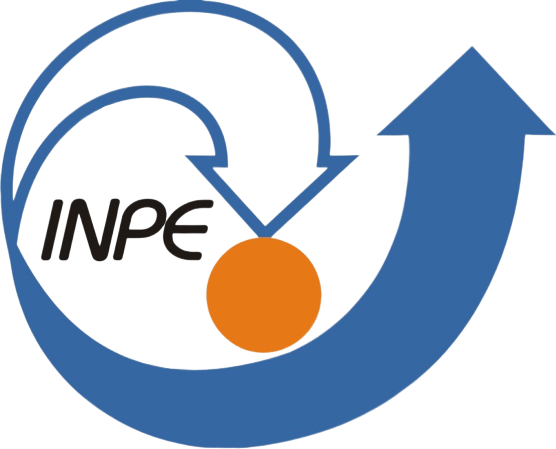
\includegraphics[width=0.21\textwidth]{img/inpe.png}
		\hfill
		
\includegraphics[width=0.35\textwidth]{img/loa.png}
		\vspace{0.3cm}
	\end{figure}
	\newcommand{\HRule}{\rule{\linewidth}{0.6mm}}
	\center
	\textsc{\LARGE Instituto Nacional de Pesquisas Espaciais}\\[0.3cm]
	\textsc{\large Laboratório de Estudos do oceano e da Atmosfera}\\[2cm]
	\HRule \\[0.7cm]
	{ \huge \bfseries \thesistitle}\\[1cm]
	\textsc{\thesissubtitle}\\
	\HRule \\[2cm]
	\begin{minipage}{.4\textwidth}
	\begin{flushleft} \large
	\emph{Beneficiário:}\\
	\thesisauthorfirst\space \textsc{\thesisauthorsecond}
	\end{flushleft}
	\end{minipage}
	\begin{minipage}{0.4\textwidth}
	\begin{flushright} \large
	\emph{Orientador:} \\
	\thesissupervisorfirst\space \textsc{\thesissupervisorsecond} \\[1em]
	\end{flushright}
	\end{minipage}\\[2.5cm]
	\textsc{\large Projeto de pesquisa apresentado à Fundação de Amparo à Pesquisa do Estado de São
	Paulo (FAPESP) com vistas à obtenção de bolsa de Doutorado}\\[3cm]
	\vfill
	{\large \thesisdate}\\
	\clearpage
\end{titlepage}

%%% Table of Contents
\hypersetup{hidelinks}
\linespread{1}
\tableofcontents\addtocontents{toc}{\protect\thispagestyle{empty}}
\clearpage
\linespread{1.5}

\renewenvironment{abstract}
{\begin{quote}
\noindent \rule{\linewidth}{.5pt}\par{\bfseries \abstractname.}}
{\medskip\noindent \rule{\linewidth}{.5pt}
\end{quote}
}

\begin{abstract}\setcounter{page}{1}
\addcontentsline{toc}{section}{RESUMO}
Em resposta à chamada CNPq/MCTIC/CAPES/FNDCT 21/2018, propomos  junto ao projeto Antartic Modeling Observation System, um projeto 
de Tese de Doutorado para investigar os processos de interação oceano-atmosfera-gelo marinho e as 
trocas de fluxos turbulentos nesta interface, em micro e mesoescalas, no Setor Atlântico do Oceano Austral. Por ser uma região
onde são necessários mais esforços para investigar o comportamento dos campos atmosféricos e hidrodinâmicos, esperamos, através
da execução deste projeto, implementar um sistema de modelagem numérica regional acoplada capaz de reproduzir com precisão e acurácia
as trocas de calor, \textit{momentum} e massa que ocorrem na interface oceano-atmosfera sob a influência da presenção ou não do gelo marinho, além
de investigar o o impacto do gelo marinho na circulação oceânica e nos processos de formação de massas d'água no Mar de Weddell. O projeto 
abrirá novos horizontes para a pesquisa do Brasil na Antártica através da modelagem numérica regional acoplada, além de fornecer dados inéditos
para propor mecanismos físicos que expliquem o papel do oceano e da atmosfera na restauração do estado de equilíbrio do gelo marinho.

\end{abstract}

%%% Introdução
\section{INTRODUÇÃO}
 \bigskip

O Oceano Austral é um importante contribuidor para a manutenção do clima da Terra. Entretanto, diversos trabalhos
apontam que o calor e o Carbono provenientes da atmosfera, bem como a ação antrópica, impactam de maneira direta neste 
ambiente. Estes impactos já são observados na região oeste da Península Antártica, com um um aquecimento de até 3 \textdegree{}C no período entre 1955 e 2004 (\cite{Turner2005})
e de cerca de 1 \textdegree{}C na porção oceânica (\cite{Meredith2015}). Apesar destes dados alarmantes, o oceano 
Austral está entre os ambientes menos compreendidos e investigados pela comunidade científica. 
Logo, devido à grande necessidade e urgência para entender as  grandes questões sobre o ambiente global da atualidade, 
são cada vez mais necessários os esforços para estudar essa região.

Desde o final da década de 80 a extensão do gelo marinho tem diminuído nos mares de Amundsen 
e Bellingshausen, sobretudo durante as estações mais quentes do ano. É observado o oposto no mar de Ross e Amundsen, 
que nas estações mais frias há um aumento da extensão do gelo marinho (\cite{Lee2017}). Estudos como 
\textcite{Parise2015}, \textcite{Cunningham2011} e \textcite{Raphael2011} investigam a interação 
gelo marinho-oceano-atmosfera e concluem que apesar da baixa troposfera ser aquecida pelos fluxos de calor
provenientes do oceano, a variação do gelo marinho na região austral pode impactar médios e altos níveis da troposfera.
Também foi estudado por \textcite{Carpenedo2013} e \textcite{Parise2015} que as variações do gelo marinho altera o 
gradiente de temperatura no eixo Equador-Polos, alterando assim o transporte meridional de calor no planeta e, como
consequência, o clima local, regional e global. Portanto, determinar as alterações no campo de gelo marinho e as causas
desta variabilidade é essencial para o melhor entendimento das variações climáticas.

Apesar desta importância, ainda são poucos os esforços para estudar o impacto do gelo marinho no clima da América do Sul.
No Hemisfério Sul, os trabalhos de \textcite{Nakamura2004} e \textcite{Ummenhofer2007} focam nas regiões da Austrália
e Nova Zelândia e o oceano Pacífico oeste. \textcite{Pook2013} comentam que quando os jatos subtropical e polar 
atigem o máximo de separação, geramente no inverno, há a ocorrência de diversos casos de eventos extremos, ligados à
bloqueios atmosféricos na Austrália e Nova Zelândia. Para a América do Sul, não há nenhum estudo que relacione a posição
do jato e eventos extremos, nem mesmo sobre a variação do gelo marinho Antártico. Recentemente, \textcite{Rodrigues2017}
mostraram que as ondas de Rossby originadas no oceano Índico e Pacífico podem vir a causar bloqueios atmosféricos 
e eventos extremos na região. Além disso, os autores comentam que a trajetória dessas ondas possuem um forte sinal na
região do mar de Amundsen, na Antártica, uma região com expressiva variação recente do gelo marinho.

Ao analisar a memória e sensibilidade do sistema climático acoplado do Hemisfério Sul ante a variação do gelo marinho, 
\textcite{Parise2015} descobriram que a restauração do equilíbrio climático após uma perturbação no gelo marinho Antártico
é desencadeada a partir de um mecanismo de dupla escala temporal, que age a partir do efeito de isolamento térmico do gelo marinho
e o consequente pulso de água doce proveniente do derretimento do gelo e restaurado pelo calor armaezando nas camadas 
subsuperficiais do Oceano Austral à medida que que a água doce e fria em superfície é advectada para latitudes mais baixas. 

Entretanto, não se conhece ainda o papel dos distúrbios transientes na restauração do balanço térmico frente à perturbações
climáticas em altas latitudes. Também não se conhece o impacto das variações na cobertura do gelo marinho Antártico nos ciclones
extratropicais na América do Sul e Atlântico Sul. 

Outra questão importante paira em torno do futuro da Corrente Circunpolar Antártica (CCA). Sabe-se que os vórtices oceânicos
de mesoescala transferem \textit{momentum} linear, de acordo com \textcite{Munk1951}, da superfície para o fundo do mar. Esse
efeito é importante para transportar calor em direção ao polo e é necessário para equilibrar o calor perdido na atmosfera embasa
altas latitudes, como estudado por \textcite{Johnson1989}. Logo, estudar o impacto que a variação do 
gelo marinho pode causar nos vórtices oceânicos é fundamental para entender um pouco mais sobre a CCA, uma vez que os
vórtices oceânicos são diretamente conectados à circulação de revolvimento global uma vez que transportam massa em 
direção aos polos em associação ao fluxo instável da CCA (\cite{Rintoul2018}). A CCA possui grande influência na 
plataforma oeste da Península Antártica. Ela flui ao longo da quebra de plataforma e é uma grande transportadora de 
calor e nutrientes através de interações com glaciares, plataforas de gelos e com uma intensa variabilidade interanual 
da formaçao e interação do gelo marinho com a atmosfera (\cite{Moffat2018}). 

No Mar de Weddell, no Setor Atlântico do Oceano Austral, está uma importante região de gelo marinho, além de ser uma fonte de massas 
de águas  frias e densas, representando uma  zona de ventilação dos oceanos e para a circulação termohalina. Estudos observacionais 
sobre a interação do gelo marinho com a atmosfera mostram que há uma forte retroalimentação entre estes dois meios, particularmente 
nas escalas de tempo mais rápidas, entretanto, o mecanismo que rege tais processos ainda não está claro. Em outras palavras, o gelo 
marinho no Oceano Austral é importante pois modifica o balanço de radiação, energia e os processos de troca de massa. 
A presença do gelo marinho reduz a Temperatura da Superfície do Mar (TSM), redireciona as correntes de superfície e altera a 
taxa de subsidência das águas de superfície nas latitudes. Como as anomalias de gelo marinho tendem a persistir por vários meses,
elas podem ter o potencial de afetar fortemente a circulação atmosférica e oceânica (\cite{Simmonds2003}).

Entre os desafios da ciência nessa região, até o presente momento a comunidade científica não conseguiu prever as respostas 
da cobertura do gelo Antártico frente às tendências climáticas devido à escassez de dados e ausência de parametrizações dos 
processos físicos que estão envolvidos nesse sistema acoplado (\cite{Turner2005}). Logo, considerando as rápidas mudanças 
no ambiente Antártico, que podem ter impactos locais, regionais e globais, percebe-se a urgência em em lançar mão 
em esforços para entender o complexo acoplamento dos mecanismos que ditam a morfologia das massas de gelo da Antártica 
(\cite{Mayewski2009}). Também é notado que não considerar a interação oceano-onda-gelo em estudos de modelagem terrestre 
é um dos motivos pelo qual os modelos climáticos não são capazes de prever a perda de gelo no continente Antártico nas últimas décadas. 
\textcite{Kohout2014} comentam que a ausência do processo de interação oceano-onda-gelo em estudos regionais e globais
é vista como uma das razões pelas quais os modelos climáticos não foram capazes de prever a perda significativa de 
massa de gelo na Antártica observada nas últimas décadas.

Outro importante desafio da ciência antártica está dificuldade na coleta de dados \textit{in situ} (\cite{Babanin2019}). 
Visto que as regiões polares são famosas por seu clima e tempo severos, a tendência para melhorar a compreensão em
estudos de interação oceano-atmosfera-gelo marinho, bem como a habilidade em modelar estas condições, é incentivar projetos que 
desenvolvam meios para obter dados de forma mais simples e barata. Recentemente, diversos estudos objetivam o desenvovimento em
eletrônicos e softwares livres e de código aberto, que criam novas oportunidades para este campo, como os trabalhos de 
\textcite{Rabault2017} e \textcite{Rabault2020}.


\subsection{Projeto AnTarctic Modeling Observation System (ATMOS)}
\bigskip

O Laboratório de Estudos do Oceano e da Atmosfera (LOA) do Instituto Nacional de Pesquisas Espaciais possui uma vasta, e antiga, cooperação com o Programa 
Antártico Brasileiro (PROANTAR). O PROANTAR foi criado em 1982 como uma resposta à entrada do Brasil no Tratado da Antártica, em 1975. É um programa
do governo brasileiro e, a partir da Comissão Interministerial para Recursos do Mar (CIRM), coordena a pesquisa e o apoio operacional para a pesquisa
na região. Atualmente o LOA/INPE conta com participação em mais de 13 Operações Antárticas (\textcolor{bleu_cite}{Figura \ref{figloa}}), através da coleta 
de dados meteorológicos e oceanográficos, que são de grande relevância na região de interesse deste projeto, e tem tido repercussão nacional e internacional. 
O grupo possui caráter multi e interdisciplinar e é composto por pesquisadores do INPE e trabalha em cooperação com diversas instituições brasileiras e 
estrangeiras, onde vários  programas de pós-graduação estão diretamente envolvidos com as pesquisas do grupo. Também é importante ressaltar este projeto
usará um cluster, com 81 nós e 2592 processadores, que o LOA/INPE possui nas dependências do Centro de Previsão de Tempo e Estudos Climáticos (CPTEC/INPE). Esse cluster
fornece uma poderosa capacidade de processamento de simulações numéricas em alta resolução e é uma ferramenta poderosa para estudos em ciência Antártica.

O Projeto ATMOS é uma iniciativa do Laboratório de Estudos do oceano e da Atmosfera do Instituto Nacional de Pesquisas 
Espaciais (LOA/INPE) e surgiu como uma resposta à chamada CNPQ/MCTIC/CAPES/FNDCT 21/2018. Foi aprovado em Novembro de 2019, 
inserido na Linha Temática "Mudanças Climáticas e o Oceano Austral". O projeto está estrutursado sob a observação \textit{in situ} 
e modelagem numérica regional acoplada para estudar os processos de Interação oceano-Ondas-Atmosfera-Gelo Marinho determinantes 
no padrão de fluxos de calor e \textit{momentum} nessas interfaces no setor do Oceano Austral. O Projeto é desenvolvido dentro
do Programa Antártico do INPE (PAN), um programa do INPE/MCTIC, e possui com parcerias em diversas instituições nacionais e 
internacionais, em particular com universidades da Inglaterra, Estados Unidos e Austrália.

O Projeto ATMOS prõpoe atingir diversos objetivos, como por exemplo:

\begin{itemize}
	\item Formar uma equipe multidisciplinar para estudar, compreender e ampliar o conhecimento científico 
	sobre os complexos processos de interação entre os subsistemas atmosfera, oceano e criosfera no Setor Atlântico
	do Oceano Austral e continentes adjacentes;
	\item Trabalhar na Iha do Rei George, onde está localizada a Estação Antártica Comandante Ferraz (EACF), visando 
	continuar os esforços do Laboratório de Estudos do oceano e da Atmosfera em estudar esta região através de projetos
	prévios como o Projeto Interação oceano-Atmosfera na Região da Confluência Brasil-Malvinas (INTERCONF);
	\item Abrir novas frentes de parcerias com universidades e institutos de pesquisa nacionais e internacionais e 
	fomentar a formação de jovens pesquisadores Antárticos brasileiros;
	\item Fomentar a inovação em projetos voltados para a aquisição de dados na Antártica a partir de dispositivos de baixo custo com 
	de código aberto e software livre.
\end{itemize}
\bigskip

A experiência adquirida na formação e condução de programas e projetos de pesquisa do Laboratório de Estudos  
do oceano e da Atmosfera (LOA), criado no âmbito da Coordenadoria de Observação da Terra (OBT) do Instituto
Nacional de Pesquisas Espaciais (INPE), embasa e motiva a apresentação do projeto ATMOS e desta proposta de tese de doutorado. 
O LOA, através do trabalho e participação científica do Coordenador, o Dr.Luciano Pezzi, contribui através de estudos 
multidisciplinares de longo prazo para o entendimento da relação entre o ambiente físico e aspectos biogeoquímicos nos oceanos
Atlântico Sul e Austral, há pelos menos 15 anos como mostrado na Figura 1 e também em vários trabalhos científicos publicados  
em revistas internacionais e nacionais. As atividades científicas desenvolvidas pelo LOA estão inseridas em inúmeros
programas nacionais e internacionais, demonstrando assim total compatibilidade com as metas de longo prazo da comunidade 
científica mundial. 

\begin{figure}[H]
    \centering
    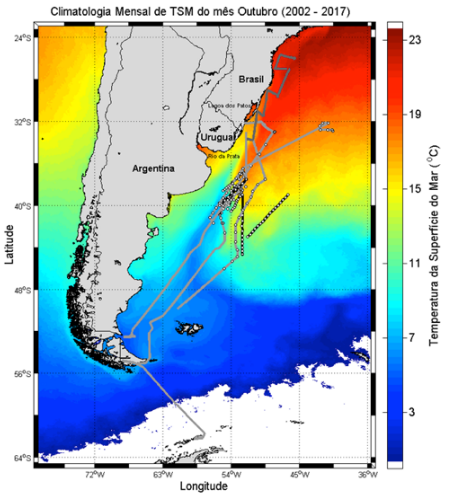
\includegraphics[width=0.60\textwidth]{img/loa_cruises.png}
	\caption{TSM climatológica do mês de outubro do satélite Aqua-MODIS entre os anos de 2002 e 2017.
	As linhas representam as trajetórias dos cruzeiros realizados
	pelo LOA-INPE entre os anos de 2004 e 2016. As linhas pretas indicam as trajetórias de
	Operações Antárticas somente com amostragens de perfis verticais de temperatura do mar e
	da atmosfera, com as posições indicadas pelos círculos brancos. As linhas cinza, indicam trajetórias de cruzeiros com
	medidas dos fluxos turbulentos.}
	\label{figloa}
\end{figure}

%%% Hipótese
\section{MOTIVAÇÃO E HIPÓTESE}
\bigskip
A partir do exposto acima, propomos lançar mão em esforços que respondam como funciona o 
acoplamento dos mecanismos de interação entre o gelo marinho-oceano-atmosfera no setor Austral do Oceano Atlântico, pois 
esta região pode sofrer alterações no balanço de trocas calor e \textit{momentum} a partir da quantidade de gelo marinho presente 
na região. Logo:
\bigskip

\textit{O gelo marinho, na região do Mar de Weddell, constitui em uma importante feição para alterar as trocas de calor e momentum entre 
o oceano e a atmosfera. Portanto, \textbf{se} houver cobertura de gelo marinho sobre o oceano, \textbf{então} os fluxos de calor latente 
e momentum na interface oceano-atmosfera serão menores que os valores encontrados quando não há essa feição. }


%%% Objetivos
\section{OBJETIVOS}
\bigskip

\subsection{Objetivo Geral}
\bigskip

Investigar os processos de interação no sistema oceano-gelo marinho-atmosfera, para compreender o efeito  
da variação temporal e espacial e o papel do gelo marinho no balanço de calor e momentum no setor Atlântico do Oceano Austral.

\subsection{Objetivos Específicos}
\bigskip

Especificamente. pretendemos atingir os seguintes objetivos específicos:

\begin{itemize}
	\item Configurar e implementar um domínio de grade numérica regional em altíssima resolução para o sistema de
	modelagem regional acoplada COAWST, com os modelos atmosférico, hidrodinâmico, de gelo marinho e o de ondas ativados;
	\item Configurar um dispositivo de baixo custo, baseado em Arduino, para a coleta de dados atmosféricos na Antártica e assimilar, 
	nas simulações, os dados coletados \textit{in situ};
	\item Realizar testes de sensibilidade e verificar o desempenho e reprodutibilidade dos modelos, comparando com
	os dados coletados durante as Operações Antárticas e de Sensoriamento Remoto;
	\item Observar o comportamento dos fluxos de calor e \textit{momentum} na presença e ausência de cobertura de gelo marinho, assim como 
	o impacto dessa feição na circulação oceânica;
	\item Estimar o efeito do gelo marinho na circulação oceânica do Mar de Weddell e a sua contribução na estratificação e formação das
	 das massas de água na região.
\end{itemize}

%%% Materiais e métodos
\section{MATERIAIS E MÉTODOS}
\bigskip

Nesta seção será apresentada a área de estudo, bem como os modelos numéricos e os dados que serão utilizados para realizar as simulações.

\subsection{Área de Estudo}
\bigskip

A Antártica é um continente com aproximadamente 14 milhões de quilômetros quadrados, marca que a coloca como o quinto maior continente
planeta (\cite{NSF2019}). Ela também abriga 90\% do gelo e 70\% da reserva total de água doce da Terra (\cite{NSF2019}). Este continente 
é circundado pelo Oceano Austral, que abriga a corrente mais importante corrente oceânica deste oceano, a CCP (\textcolor{bleu_cite}{Figura \ref{meridional}}), que flui de oeste para leste
e possui transporte médio entre 100-150 Sverdrups e temperatura média variando entre -1 a 5 \textdegree{}C, dependendo da época do ano e
localização e os valores típicos de salinidade variam entre 33.5 e 34.7 em direção à 65 \textdegree{}S.
Esta assinatura de temperatura e salinidade é devida a combinação de massas de água que se encontram no Oceano Austral e são misturadas e 
redistribuídas pela CCP (\cite{Pickard1990}).
\bigskip

\begin{figure}[H]
    \centering
    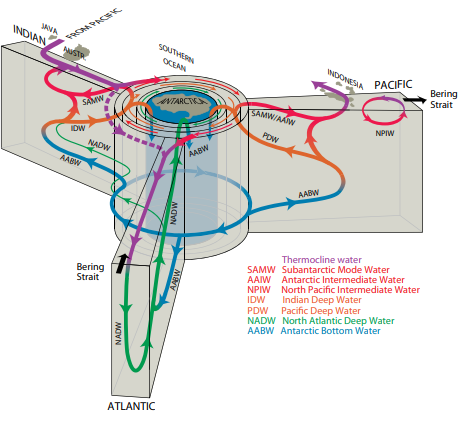
\includegraphics[width=0.60\textwidth]{img/meridional.png}
	\caption{Representação esquemática da Célula de Revolvimento Global proposta por \textcite{Talley2013}. Observa-se a formação da AABW na região
	do Mar de Weddell.}
	\label{meridional}
\end{figure}


O Oceano Austral é essencial para investigações sobre o estudo climático do planeta, pois é o principal meio onde ocorrem as trocas de calor,
energia e massa entre as três principais bacias oceânicas do planeta. Além disso, a variabilidade sazonal e interanual da cobertura do gelo 
marinho ocasionam um significativo impacto nos processos de formação de massas de água, em particular no mar de Weddell, onde é formada a 
Água de Fundo antártica (AABW; \cite{Santini2018}; \cite{Talley2013}). A AABW (\textcolor{bleu_cite}{Figura \ref{meridional}}) é formada, 
de acordo com \cite{Talley2013},  a partir da geração de massas de água profundas e com alta salinidade
em altas latitudes do Atlântico Norte (NADW) e que são transportadas em direção ao hemisfério sul pela Célula de Revolvimento Meridional do Atlântico (AMOC) 
e que ganha calor durante sua trajetória e ascende à superfície no Oceano Austral. \textcite{Santini2018}, \textcite{Haid2013} e \textcite{Tamura2011} comentam que a formação da AABW também está associada
à formação do gelo marinho e seu derretimento sazonal, que influenciam a estabilidade do oceano superior devido à mudança da salinidade associada ao efeito Brine\footnote{Liberação do sal para o meio líquido durante a formação do gelo marinho.}. 
\bigskip

\subsubsection{O Mar de Weddell}
\bigskip

 A porção ao leste da Península Antárticar possui como mais importante feição o Giro de Weddell (GW). Conforme observado na Figura \textcolor{bleu_cite}{Figura \ref{weddell}}, ele é um giro ciclônico 
(move-se no sentido oeste no ramo sul e para leste no ramo norte) que encontra na ação dos ventos a sua maior força motriz. De acordo com 
\textcite{Gordon2001}, essa região possui um grande transporte ascendente de água de subsuperfície no interior do giro, 
devido a um forte bombeamento de Ekman ocasionado pela natureza divergente do giro. A região também é formadora da Água Circumpolar Profunda (CDW),
formada nas partes sule oeste do GW, em regiões próximas à Península Antártica e a água em superfície é trocada a pela proximidade com a CCA (\cite{Vernet2019}). 
A CDW possui temperatura máxima logo abaixo da picnoclina, de acordo com \textcite{Kerr2018}, e os maiores valores de temperatura são encontrados na região sudeste do GW, 
indicando essa região como um importante local recipiente de água da CCA.
\bigskip

  A produção de água mais densa deve ocorre, preferencialmente, na Plataforma Continental na porção sudoeste do Mar de Weddell, onde a água é
é resfriada para o ponto de congelamento devido ao contato com a atmosfera, e aumenta a salinidade, a partir da expulsão do sal durante o congelamento a partir do efeito Brine 
(\cite{Vernet2019}). A partir desse processo, a água segue para a margem da Plataforma Continental e flui em direção ao assoalho oceânico até ser desviada à esquerda,
 pelo efeito de Coriolis, e é incorporada ao GW.
\bigskip


\begin{figure}[H]
    \centering
    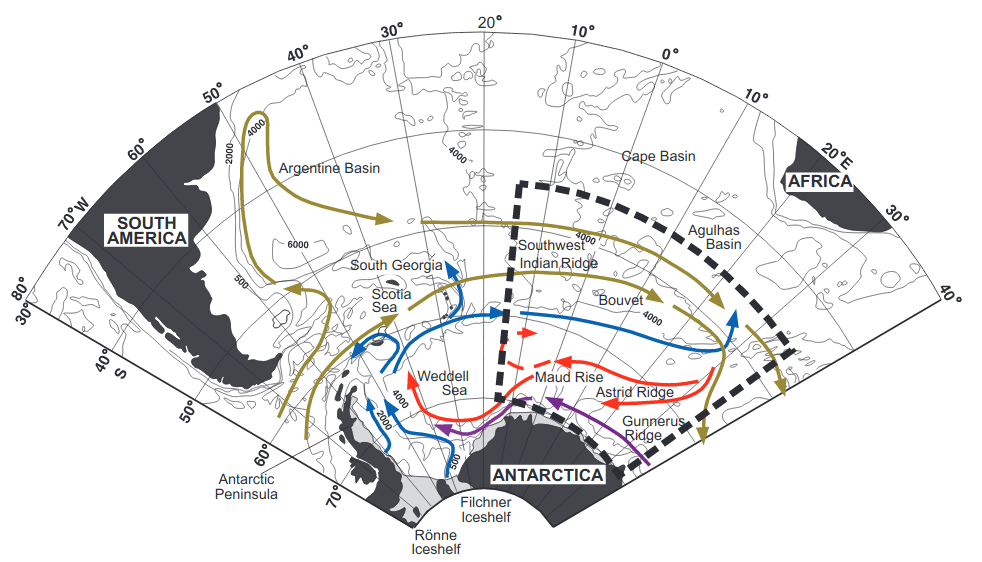
\includegraphics[width=1\textwidth]{img/weddell.png}
	\caption{Representação esquemática da circulação profunda da CDW(linhas vermelhas). A Corrente costeira Antártica está representada pelas linhas de cor roxa, e a formação e circulação da CDWoriginada no lado leste da Plataforma Antártica,está representada pelas linhas azuis.}
	\label{weddell}
\end{figure}
\bigskip

\subsection{Modelos numéricos}
\bigskip

Nesta subseção serão descritos os modelos numéricos que serão utilizados para a execução deste projeto.

\subsubsection{Weather Research Forecast (WRF)}
\bigskip

O WRF (\cite{Skamarock2008}) é um modelo atmosférico desenvolvido pelos National Centers for Environmental Prediction (NCEP), 
National Center for Atmospheric Research (NCAR) e grupos de pesquisa de diferentes universidades. Para integrar 
no tempo as equações governantes, o módulo Advanced Research WRF (ARW) utiliza modos de baixa freqüência que 
são integrados utilizando o esquema de Runge-Kutta de terceira ordem, e os modos acústicose de ondas de gravidade 
(alta frequência) integrados com menor passo de tempo. Dessa maneira, se mantém aestabilidade numérica, 
através de um esquema \textit{forward-backward} para os modos acústicos que se propagam horizontalmente, e de um esquema 
implícito para modos acústicos de propagação vertical e oscilações de empuxo (\cite{Skamarock2008}). O modelo WRF 
utiliza uma grade do tipo Arakawa-C (\cite{Arakawa1977}), onde as velocidades normais são escalonadas a meio 
comprimento da grade das variáveis termodinâmicas.

\subsubsection{Regional Ocean Modeling System (ROMS)}
\bigskip

O ROMS (\cite{Shchepetkin2005}) é um modelo oceânico tridimensional de superfície livre, 
coordenada vertical sigma (seguidora do terreno) e que resolve equações primitivas. Este modelo utiliza a média de 
Reynolds e o método de diferenças finitas para resolver as equações de Navier-Stokes, assumindo aproximações hidrostáticas
e de Boussinesq (\cite{Haidvogel2008}). As equações hidrostáticas de \textit{momentum} utilizam um esquema de passo de tempo 
\textit{split-explicit}, onde os modos barotrópico e baroclínico são resolvidos separadamente e em distintos números 
finitos de passos de tempo para resolver as equações de superfície livre e \textit{momentum} integrado na vertical. 
Esta estrutura separada de passos de tempo separados mantém a conservação de volume e a preservação de consistência que são necessárias 
para as equações de traçadores (\cite{Haidvogel2008}; \cite{Shchepetkin2005}). A partir da grade, o modelo resolve 
as equações na horizontal através de coordenadas curvilíneas ortogonais do tipo Arakawa-C (\cite{Arakawa1977}). 
Na vertical, as coordenadas seguem as feições do terreno e permitem ajustar a resolução ao longo da coluna d’água. 
Para garantir a conservação de \textit{momentum}, a grade utiliza diferenças finitas de segunda ordem (\cite{Haidvogel2008}).

\subsubsection{Simulating Waves Nearshore (SWAN)}
\bigskip

O SWAN (\cite{Booij1996}; \cite{Booij1999}) é um modelo de terceira geração, concebido
para uso em regiões costeiras com águas rasas e correntes locais. O modelo é amplamente utilizado na
previsão numérica do espectro de ondas em regiões costeiras, estuários, canais e outros, podendo utilizar
campos de vento, batimetria e correntes fornecidos por outros modelos (\cite{Booij1996}; \cite{Booij1999}).

\textcite{Dasilva2013}, \textcite{Booij1996} e \textcite{Booij1999} elencam as principais características do SWAN:

\begin{itemize}
	\item Refração de onda com profundidade variável;
	\item Empinamento induzido pela profundidade e corrente;
	\item Geração e propagação de ondas pelo vento;
	\item Dissipação por \textit{whitecapping};
\end{itemize}

\subsubsection{Budgell's Sea Ice Model}
\bigskip

O Modelo de Gelo Marinho, proposto por \textcite{Budgell2005} está integrado ao modelo oceânico ROMS
e compartilha os mesmos passos de tempo e grade do modelo, além da mesma estrutura de codificação paralela para 
uso com Message Passing Import (MPI). Dessa maneira, permite a modelagem dinâmica e termodinâmica onde houver o 
predomínio de gelo marinho,como por exemplo em altas latitudes. Os principais atributos do modelo, de acordo com 
\textcite{hedstrom2018}, são:

\begin{itemize}
	\item Dinâmica elástica-viscosa de \textcite{Hunke1997} e \textcite{Hunke2001};
	\item Termodinâmica proposta por \textcite{Mellor1989};
	\item Coordenadas curvilíneas-ortogonais;
	\item Grade Arakawa-C proposto por \textcite{Arakawa1977};
	\item Advecção de traçadores proposta por \textcite{Smolarkiewicz1990};
	\item Parametrização de gelo proposta por \textcite{Lemieux2015}.
\end{itemize}

\subsubsection{Model Coupling Toolkit (MCT)}
\bigskip

O MCT (\cite{Jacob2005}; \cite{Larson2005}; \cite{Warner2008}) é um conjuntode rotinas livres, escritas em Fortran 90 que 
permitem a transmissão e transformação dos diferentes dadosnecessários ao acoplamento de modelos. Durante a inicialiação, 
os domínios dos modelos são decompostosem segmentos que são distribuídos entre os processadores, permitindo que os 
modelos sejam acopladostambém de forma paralela.

\begin{itemize}
	\item Um registro das componentes dos modelos;
	\item Descritores de decomposição do domínio;
	\item Ferramentas paralelizadas para interpolação entre grades;
	\item Feramentas para mesclar dados de entre vários componentes;
	\item Um modelo de programação semelhante ao MPI (Message Passing Interface).
\end{itemize}

\subsubsection{Spherical Coordinate Remapping Interpolation Package (SCRIP)}
\bigskip

O SCRIP (\cite{Jones1998}; \cite{Jones1999}) é um pacote necessário para projetos que utilizam mais de um modelo numérico e que possuem 
grades horizontais diferentes, ou seja com diferentes resoluções espaciais. O SCRIP gerará os pesos de interpolação que serão usados 
para remapear os dados entre as distintas grades dos diferentes modelos, para que haja o acoplamento e troca de informação entre os modelos numéricos.

\subsubsection{Coupled Ocean Atmosphere Wave Sediment Transport Modeling System (COAWST)}
\bigskip

O COAWST é um sistema \textit{open-source} de modelagem numérica regional acoplada composto pelos módulos atmosférico, oceânico, ondas e de sedimentos oceânicos. 
O modelo atmosférico é o WRF, o modelo oceânico é o ROMS, o modelo de ondas são o SWAN ou o WaveWatch 3  e o modelo de transporte de sedimentos é o Community 
Sediment Transport  Modeling  Project (CSTM; \cite{Warner2008}). O COAWST, é um sistema baseado no conceito de “modelo de comunidade”, ou seja,
é desenvolvido por um grupo de pesquisadores de várias instituições internacionais, como  mostrado  no trabalho de \textcite{Warner2010}.
Esse  sistema, permitiu os avanços na representação da dinâmica costeira, devido ao acoplamento do modelo de ondas ao de circulação  oceânica e
atmosférica (\cite{Warner2008}). Um aspecto do COAWST que deve ser ressaltado, é que ele permite um acoplamento dinâmico   
entre o oceano e a atmosfera aonde os fluxos são trocados ativamente nas duas direções, da atmosfera 
para o oceano e vice-versa. Esses modelos tridimensionais têm sido desenvolvidos e aplicados a cenários idealizados 
para se entender alguns processos de maneira isoladae em cenários realistas, como simular as interações entre um ciclone 
tropical e o oceano (Bender e  Ginis,  2000;  Bender  et  al,  2007;  Chen  et  al,  2007).  

O COAWST, através do MCT (\cite{Jacob2005}), permite a troca 
de informações entre os modelos com uma frequência ajustável definida pelo usuário. Para o presente projeto de tese de doutorado, 
escolheremos o modelo de ondas SWAN como modelo de ondas e ativaremos todos os outros modelos, com excessão
CSTM. A utilização do COAWST, como sistema de modelagem numérica, possibilitará a simulação mais acurada e precisa
dos processos de interação oceano-atmosgera-gelo marinho, permitindo identificar a evolução da dinâmica e termodinâmica
da região de estudo.

 Conforme a \textcolor{bleu_cite}{Figura \ref{acopla}}, as informações trocadas entre modelos são:

\begin{itemize}
\item WRF para o ROMS: cisalhamento de superfície e fluxo de calor líquido (calculado no ROMS a partir das componentes dos fluxos de calor latente e sensível e radiação de ondas curta e longa, a pressão atmosférica, umidade relativa, temperatura do ar, nuvens, precipitação e as componentes do vento;
\item ROMS para o WRF: temperatura da superfície do mar;
\item SWAN para o ROMS: direção da onda em superfície e no fundo, altura, comprimento, período, dissipação de energia e velocidade orbital inferior;
\item ROMS para o SWAN: batimetria, elevação da superfície, altura da superfície do mar e correntes médias em profundidade;
\item SWAN para o WRF: rugosidade da superfície do mar (calculado no WRF a partir da altura significativa da onda, comprimento e período);
\item WRF para o SWAN: vento em 10m de altura.
\end{itemize}
\bigskip

\begin{figure}[H]
	\hspace*{-1.7cm}
    \begin{tikzpicture}[->,
        >=stealth',
        shorten >=1pt,
        auto,
        node distance=2.75cm, 
        state/.style={
        draw=black,
        fill=bashcodebg,
        circle, 
        text=black,
        text width={width("ROMS")},
        minimum size=1.5cm,
        align=center,
        rounded corners,
        font=\small}]

        \hspace{5cm}
        \node[state] (A)  {\small WRF};
        \node[state] (C)  [right=4cm of A] {\small ROMS \scriptsize{Sea ice}};
        \node[state] (B)  [below=4cm of C,right of= A] {\small SWAN};

        \path (A) edge [draw=black, bend right=20] node[sloped, align=center, below,font=\tiny]  {U\textsubscript{wind}, V\textsubscript{wind}, P\textsubscript{atm}, RH, \\T\textsubscript{air}, Cloud, Rain, \\SW\textsubscript{rad}, LW\textsubscript{rad}} (C); % WRF->ROMS
        \path (C) edge [draw=black, bend right=20] node[sloped, align=center, below,font=\tiny] {SST} (A);
        \path (A) edge [draw=black, bend right=20] node[sloped, align=center, below,font=\tiny] {U\textsubscript{wind}, \textsubscript{wind}} (B); 
        \path (B) edge [draw=black, bend right=20] node[sloped, align=center, below,font=\tiny] {L\textsubscript{wave}, H\textsubscript{wave}} (A);
        \path (B) edge [draw=black, bend right=20] node[sloped, align=center, below,font=\tiny] {L\textsubscript{wave}, H\textsubscript{wave}, D\textsubscript{wave}, \\T\textsubscript{surface}, T\textsubscript{bottom}, Q\textsubscript{B}, \\W\textsubscript{dissipation}, U\textsubscript{b}} (C); 
        \path (C) edge [draw=black, bend right=20] node[sloped, align=center, below,font=\tiny] {U\textsubscript{s}, V\textsubscript{s}, Bathymetry, \\Bottom Elevation} (B); 
        \node[align=center,font=\bfseries, yshift=2em] (title) at (current bounding box.north) {\small Coupled Ocean-Atmosphere-Wave-\\\small Sediment Transport modeling system};
	\end{tikzpicture}
\caption{Esquema da troca de informações entre três modelos que compõe o sistema COAWST (Adaptado de \textcite{Warner2008}; fonte: \textcite{Sutil2019b}).}
\label{acopla}
\end{figure}

Existem diversos estudos publicados que utilizam o COAWST. \textcite{Warner2008} mostraram a estrutura do COAWST e sua aplicação na simulação do 
furacão Isabel, ocorrido  em  setembro  de  2003. Para isso foi realizada  uma sequência de simulações, alterando-se as componentes do 
sistema de modelagem e o modo de acoplamento entre os módulos atmosfera-oceano-ondas e foi mostrado que a simulação do fenômeno foi mais acurada e precisa ao
utilizar o acoplamento entre modelos. Recentemente \cite{Pullen2018}, apresentaram uma interessante revisão sobre estutruradas de modelagem acoplada, onde foram simulados
alguns estudos de caso de interação oceano-atmosfera para investigar o o acoplamento entre ciclones tropicais e o oceano, como o primeiro furacão híbrido
ocorrido no oceano Atlântico, o Catarina (\cite{McTaggart2006}).


\subsection{Dados}
\bigskip

Nessa subseção serão apresentados os dados que serão utilizados para alimentar o sistema de modelagem numérica para realização das simulações.

\subsubsection{Dados \textit{in situ} do LOA/INPE}
\bigskip

O LOA/INPE possui um extenso banco de dados \textit{in situ}, com mais de 13 anos de coletas (\textcolor{bleu_cite}{Figura \ref{figloa}}) no Oceano Austral e
Atlântico utilizando CTS, XBTs, bóias oceanográficas, flutuadores,radiossondagens da atmosfera e de fluxos turbulentos que poderão ser utilizados 
como comparação com as simulações realizadas pelos modelos. 

Para este projeto de tese de doutorado, utilizaremos os dados meteoceanográficos coletados entre Outubro e Novembro de 2018, durante a Operação Antártica 37 
e entre Outubro e Dezembro de 2019, durante a Operação Antártica 38, para verificar o desempenho dos modelos em simular as condições atmosféricas e oceânicas 
da região de estudo.


\subsubsection{Dispositivo de Baixo Custo para Coleta de Dados Atmosféricos (DBCCDA)}
\bigskip
A fim de incentivar o fomento à inovação na pesquisa Antártica e lançar mão nos esforços para coleta de dados em uma região com condições severas
de tempo e clima, pretendemos construir um Dispositivo de Baixo Custo para Coleta de Dados Atmosféricos (DBCCDA), baseado em Arduino e com software livre e de 
código aberto. Os dados deste dispositivo serão acrescentados ao banco de dados criado pelo LOA/INPE e serão usados na assimilação de dados dos 
modelos numéricos.
\bigskip

Para o desenvolvimento do DBCCAA, utilizamos uma placa de desenvolvimento DOI ESP32 ESP-WROOM-32, produzida pela Doctors of Intelligence Technology (DOIT). 
Baseado no CHIP ESP32-D0WDQ6, feito pela empresa Espressif, a placa possui funções que incorpora a utilização de WiFi, Bluetooth e o microprocessador, 
que a qualifica para atender uma grande variedade de projetos. O ESP32 possui um microprocessador Xtensa 32-Bits LX6 de baixo consumo de
energia, com dois núcleos de CPU (processador dual core) que podem ser controlados individualmente com frequência de clock ajustável de 80MHz à 240MHz. 
Outra vantagem é a possibilidade de desligar a CPU e utilizar o co-processador de baixa potência para monitorar, com baixo consumo de energia, periféricos 
como sensores e interfaces I2C.
\bigskip

Para a coleta de dados de Temperatura do Ar e Umidade Relativa, escolhemos o sensor DHT/AM3202, que utiliza um sensor
de umidade capacitativo e um termistor para medir o ar circundante e converte o dado obtido através da emissão de um sinal digital, sem a necessidade de
conversores analógicos. Com baixo custo, o sensor permite obter leitura de dados a cada 2 segundos (0,5 Hz). A faixa de medição do sensor de umidade é de 
0 a 100\%, com precisão de 2-5\% e a faixa de midção de temperatura é de -40 a 80 \textdegree{}C, com 0.5 \textdegree{}C de
precisão.
\bigskip

Para os dados de Pressão Atmosférica, utilzamos o sensor BME280 desenvolvido pela Bosch. Ele é um sensor que mede de 0 a 100\%
com precisão de 3\% a umidade relativa, pressão barométrica de 300Pa a 1100 hPa com precisão absoluta de1 hPa e temperatura de -40 \textdegree{}C a 
85\textdegree{}C com precisão de 1\textdegree{}C.
\bigskip

Atualmente o dispositivo encontra-se em fase de desenvolvimento, com um teste realizado durante a Operação Antártica 38, em Fevereiro de 2020, 
conforme apresentado na \textcolor{bleu_cite}{Figura \ref{dbccda}}. No futuro, pretendemos acoplar um sensor de magnitude de vento junto ao dispositivo.

\bigskip

\begin{figure}[H]
    \centering
    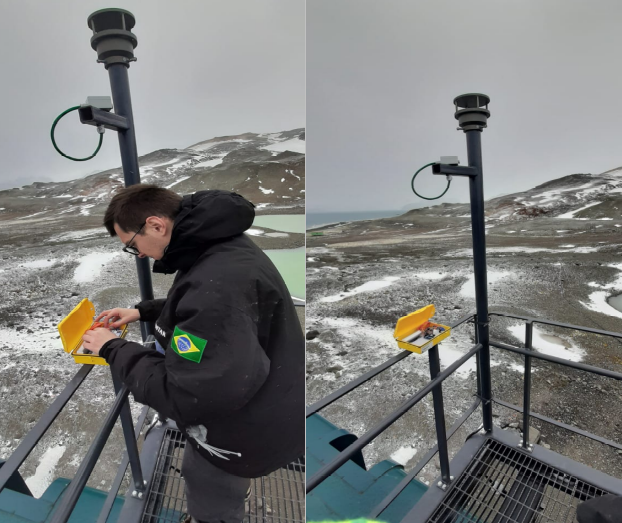
\includegraphics[width=0.70\textwidth]{img/dbccda.png}
	\caption{Beneficiário do projeto testando o DBCCDA na Baía do Almirantando durante a Operação Antártica 39, em Fevereiro de 2020.}
	\label{dbccda}
\end{figure}
\bigskip

\subsubsection{NOAA/NSDIC Climate Data Record of Passive Microwave Sea Ice Concentration (CDR)}
\bigskip

Com uma resolução espacial de 25 x 25 km, o CDR (\cite{Peng2013}) fornece os registros de concentração de gelo marinho obtidos a partir de sensores passivos de micro-ondas instalados em satélites. O banco de dados
fornece uma série temporal consistente, diária e mensal de concentrações de gelo do mar, de 09 de julho de 1987 até o processamento mais recente nas duas
regiões polares do planeta. Estes dados, assim como os dados obtidos pelo LOA/INPE serão utilizados como fonte de comparação com as simulações realizadas pelo 
COAWST.

\subsubsection{ERA5 Reanalysis Dataset}
\bigskip

ERA5 (\cite{ERA5}) é uma reanálise produzida pelo European Centre for Medium-Range Weather Forecasts (ECMWF). Ele cobre o período
de Janeiro de 1950 até a atualidade e é distribuído com 37 níveis de pressão, da superfície até 0.01 hPa. A resolução
espacial é de 31 km e a resolução espacial é horária e mensal. Os dados do ERA5 serão utilizados para alimentar as forçantes do modelo atmosférico WRF.

\subsubsection{Simple Ocean Data Assimilation (SODA) v3.12.1}
\bigskip

O SODA v3.12.1 (\cite{Carton2018}) é um conjunto de reanálise que utiliza
um modelo de circulação geral dos oceanos com resolução horizontal de 0.25ºx0.25º e 40 níveis verticais seguidoras
do terreno e a resolução temporal é de 5 ou 10 dias ou mensal, disponível entre 1980 e 2015.
O SODA possui variáveis bidimensionais da altura do nível do mar, componentes zonal e meridional da 
velocidade integrada na vertical e variáveis tridimensionais de temperatura, salinidade, componente zonal e meridional
da velocidade e variáveis de gelo marinho. Os dados do SODA serão utilizados para alimentar as forçantes do modelo hidrodinâmico ROMS.

\subsubsection{ETOPO1 1 Arc-Minute Global Relief Model (ETOPO1)}
\bigskip

O ETOPO1 (\cite{Amante2009}) é produzido pelo National Geophysical Data Center e fornece duas camadas de informações 
de relevo. As camadas incluem batimetria sobre os oceanos e algunsdos principais lagos da Terra. A topografia terrestre 
e a batimetria oceânica baseiam-se na topografia SRTM30e através de vários cruzeiros batimétricos. Os dados do ETOPO1 serão utilizados 
para alimentar a grade batimétrica utilizada pelo modelo hidrodinâmico ROMS.

\subsection{Preparação e Análise dos Dados}
\bigskip

Nessa seção serão descritos como os dado serão preparados para realizar as simulações bem como a análise dos dados obtidos.

\subsubsection{Realização das Simulações}
\bigskip

Nessa seção serão descritas como serão realizadas as simulações, com suas respectivas avaliações e análises.

\subsubsection{Planejamento dos experimentos}
\bigskip

A fim de representar as principais características meteoceanográficas da área de estudo, propomos a realização os seguintes experimentos:
\bigskip

\begin{itemize}
	\item \textbf{CTRL}: Experimento controle realizado com a assimilação de dados \textit{in situ};
	\item \textbf{CTRL\_NO\_INSITU}: Experimento controle sem a assimilação de dados;
\end{itemize}
\bigskip

Após a realização dos três experimentos, os dados simulados serão avaliados utilizando  dados \textit{in  situ} provenientes das coletas do projeto ATMOS.
Os dados atmosféricos para pressão, umidade relativa, direção e velocidade do vento e temperatura do ar serão comparados com os dados das radiossondagens, os dados oceânicos 
para temperatura serão comparados com dados  de XBT, CTD e a bóia oceanográfica, e, por fim, os dados de gelo marinho serão comparado com dados do CDR. 
As avaliações serão conduzidas com  a produção de diagramas de Taylor (\cite{Taylor2001}). Esse diagrama é eficiente em identificar a Raiz 
Quadrada do Erro-Médio (RMSE), o desvio padrão do experimento e o coeficiente de correlação. Também serão gerados mapas horizontais 
do RMSE, viés e Erro Médio Absoluto.
\bigskip

As equações do RMSE (1) e do Viés (2) são mostradas abaixo:
\bigskip

\begin{equation}
	RMSE = \sqrt{\frac{\sum_{i}^{n}(X_{sim,i}-{X_{obs,i}})^2}{n}}
\end{equation}
\bigskip

\begin{equation}
	Vies = \sum_{i}^{n}(X{_{sim}-X_{obs}})
\end{equation}
\bigskip

Onde: 
\bigskip

\textit{X\textsubscript{sim}} é a variável simulada e \textit{X\textsubscript{obs}} é a variável observada e \textit{n} é o número amostral.
\bigskip

Pretende-se, com essa metodologia, ser capaz de avaliar se a assimilação de dados apresentou um incremento significativo na capacidade de simular a região de estudo ante ao 
experimento sem a assimilação. 
\bigskip

Após a verificação da performance de cada simulação (CTRL e CTRL\_NO\_INSITU), será utilizada a simulação que melhor representou a região de estudo para ser
analisada com os próximos experimentos que modificarão a quantidade de gelo marinho presente no Mar de Weddell. Os experimentos são:
\bigskip

\begin{itemize}
	\item \textbf{ICE\_NORMAL}: Simulação com a presença de gelo marinho;
	\item \textbf{ICE\_MINUS\_100}: Simulação sem o de gelo marinho presente na simulação ICE\_NORMAL;;
	\item \textbf{ICE\_MINUS\_80}: Simulação com 80\% menos de gelo marinho presente na simulação ICE\_NORMAL;
	\item \textbf{ICE\_MINUS\_60}: Simulação com 60\% menos de gelo marinho presente na simulação ICE\_NORMAL;
	\item \textbf{ICE\_MINUS\_40}: Simulação com 40\% menos de gelo marinho presente na simulação ICE\_NORMAL;
	\item \textbf{ICE\_MINUS\_20}: Simulação com 20\% menos de gelo marinho presente na simulação ICE\_NORMAL;
	\item \textbf{ICE\_SUM\_100}: Simulação com 100\% menos de gelo marinho presente na simulação ICE\_NORMAL;
	\item \textbf{ICE\_SUM\_80}: Simulação com 80\% menos de gelo marinho presente na simulação ICE\_NORMAL;
	\item \textbf{ICE\_SUM\_60}: Simulação com 60\% menos de gelo marinho presente na simulação ICE\_NORMAL;
	\item \textbf{ICE\_SUM\_40}: Simulação com 40\% menos de gelo marinho presente na simulação ICE\_NORMAL;
	\item \textbf{ICE\_SUM\_20}: Simulação com 20\% menos de gelo marinho presente na simulação ICE\_NORMAL;
\end{itemize}
\bigskip

Para avaliar a simulação ICE\_NORMAL, será aplicada a mesma metodologia utilizada na definição da simulação controle.
\bigskip


\subsubsection{Grades e aninhamento}
\bigskip
Para o modelo atmosférico, será utilizado um domínio de alta resolução no Oceano Austral para aninhar outros dois subdomínios
menores e de maior resolução espacial (dividos por um fator de 3), conforme a (\textcolor{bleu_cite}{Figura \ref{wrfdomain}}). 
Para os modelos oceânico, de ondas e de gelo marinho, propomos apenas um domínio para cada modelo, semelhantes ao domínio d01 
do modelo atmosférico.
\bigskip

\begin{figure}[H]
    \centering
    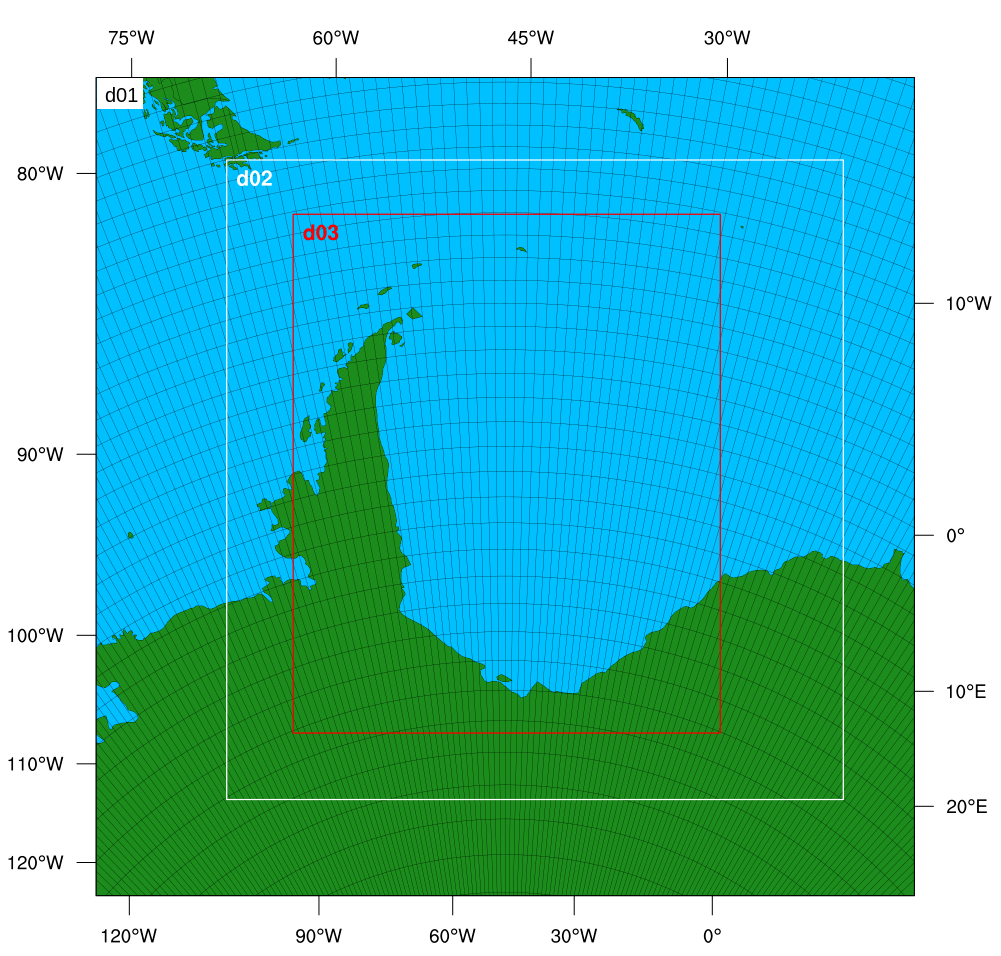
\includegraphics[width=0.50\textwidth]{img/domainswrf.png}
	\caption{Representação esquemática dos domínios propostos (d01, d02 e d03) para as simulações no modelo atmosférico.}
	\label{wrfdomain}
\end{figure}

Quanto à resolução espacial, propomos utilizar na primeira grade (d01) no modelo atmosférico, 30 km x 30 km, na segunda grade (d02), 
10 km x 10 km e na terceira grade (d03), 3.33 km x 3.33 km. As grades dos modelos hidrodinâmico, de ondas e de gelo marinho terão 
8 km x 8 km de resolução espacial.
\bigskip


\subsubsection{Estimativas de Fluxo de Calor}
\bigskip

Propomos estimar os Fluxos de Calor Latente (\textit{Q\textsubscript{L}}) e Sensível (\textit{Q\textsubscript{S}}) descritos em \textcite{Pezzi2009} e \textcite{Fairall1996}
e apresentados abaixo:

\begin{equation}
Q_{S} = \rho c_{p}C_{h}U(\theta_{air}-SST)
\end{equation}

\begin{equation}
Q_{L} = \rho L_{e}C_{e}U(q_{s}-q_{air})
\end{equation}
\bigskip

Onde \textit{C\textsubscript{h}} e \textit{C\textsubscript{e}} são os coeficientes de transferência de calor e umidade que dependem dados
estabilidade atmosférica e são gerados por relações de similaridade. \textit{$\theta$\textsubscript{air}} é a temperatura potencial,
\textit{q\textsubscript{s}} é a umidade específica ao nível do mar e \textit{q\textsubscript{air}} é a umidade específica em \textit{z\textsubscript{r}}.
\textit{U} é a velocidade média dos ventos em superfície relativos à superfície do mar. Propomos estudar também o Fluxo Total de Calor (\textit{Q\textsubscript{T}}), dado por:

\begin{equation}
	Q_{T} = Q_{L} + Q_{S}
\end{equation}
\bigskip

Esses cálculos são realizados com base em parametrizações aerodinâmicas (\textit{bulk}) do
esquema proposto por \textcite{Fairall2003}.  \textcite{Vihma2002} estudou o balanço de calor no Mar de 
Weddell, comparando  dados  coletados por boias ancoradas e saídas de modelo. Com a possibilidade de medir 
diretamente os fluxos de calor sensível e latente a partir dos sensores instalados em uma torre  
micrometeorológica, que já está sendo largamente utilizada pelo projeto ATMOS e nas  campanhas anteriores do LOA/INPE, 
o próprio método de parametrização pode ser melhor avaliado para a região desse estudo, além de servir de  
base para avaliação  dos  dados  simulados. \textcite{Santini2018} e \textcite{Butterworth2016} mostraram  
que o fluxo de calor latente em médias e altas  latitudes podem apresentar divergências em suas  magnitudes 
de acordo  com o método utilizado para sua determinação (\textit{bulk} ou  covariância de vórtices) associados a diferentes 
condições ambientais.

%%% Resultados
\section{RESULTADOS}
\bigskip

Nessa seção serão apresentados resultados preliminares do projeto e os resultados previstos para a conclusão da tese de doutorado.

\subsection{Resultados Preliminares}
\bigskip

\subsubsection{Simulação preliminar}
\bigskip

Este projeto completa uma realização de uma simulação teste para a região de interesse. Utilizando o sistema de modelagem numérica
regional acoplado COAWST, realizados uma simulação entre os dias 01 de Setembro e 01 de Outubro de 2015. 
A \textcolor{bleu_cite}{Figura \ref{figroms}A} apresenta a TSM e os vetores das correntes oceânicas em superfície para o último dia da
simulação. É possível observar feições características da região, como a CCA, além de valores de temperatura próximas às encontradas na 
literatura científica. 

A \textcolor{bleu_cite}{Figura \ref{figroms}B} apresenta um corte longitudinal da TSM e temperatura do ar entre 55 \textdegree{}S e 64 \textdegree{}S na longitude de 
66 \textdegree{}O. É possível observar a interação oceano-atmosfera da região, com a modulação local da atmosfera através do oceano: em regiões
onde o oceano está com uma temperatura mais quente, há a presença de temperatura do ar mais quente e vice e versa.
\bigskip

\begin{figure}[H]
    \centering
    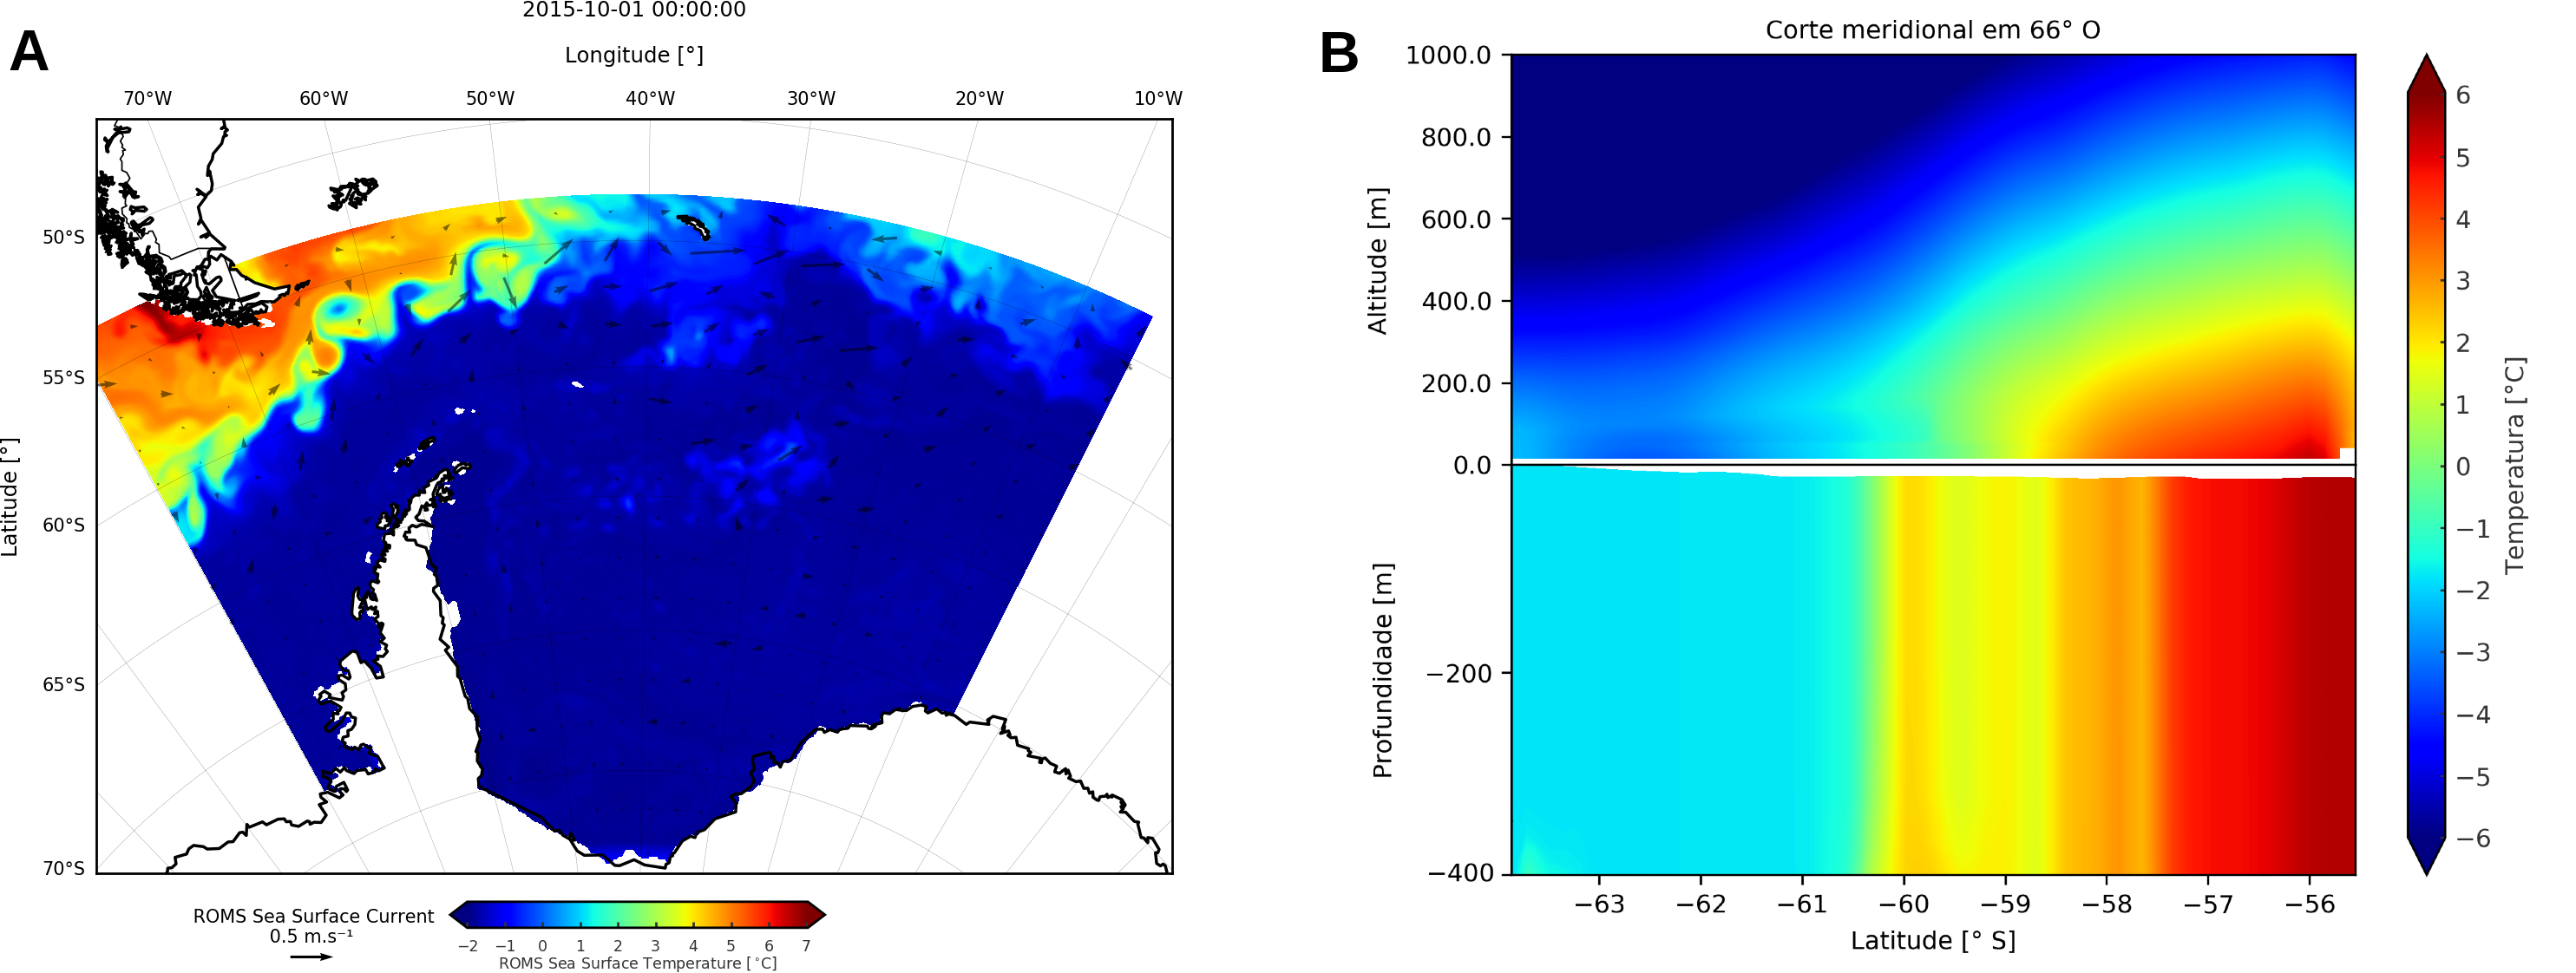
\includegraphics[width=0.7\textwidth]{img/wrf_roms.png}
	\caption{Simulação-teste realizada para o dia 01 de Outubro de 2015. (A) Temperatura da Superfície do Mar (colorido; \textdegree{}C) e Correntes Oceânicas de Superfície (vetores; m/s). (B) Temperatura do Ar (colorido; \textdegree{}C) e Temperatura do Mar (colorido; \textdegree{}C.) 
	}
	\label{figroms}
\end{figure}

A simulação teste foi realizada para avaliar a capacidade de reproduzir uma simulação para a região de interesse. 
Ressalta-se que o proponente publicou em setembro de 2018 o Guia Prático para Utilização do COAWST (\cite{Sutil2018}), um guia que foi 
desenvolvido para auxiliar novos usuários com a familiarização e utilização do COAWST. O Guia foi planejado para ensinar ao leitor as 
etapas necessáriias para utilizar o COAWST, da instalação do modelo à simulação de um caso teste e a configuração de um projeto. Em 
setembro de 2019, foi publicada a segunda edição do Guia Prático para COnfiguração do COAWST (\cite{Sutil2019b}), com a atualização para a versão 3.4 do COAWST, a Introdução
de um capítulo sobre o modelo de gelo marinho e a remodelação do pacote de ferramentas \textit{model2roms} utilizado para gerar os dados de 
entrada do modelo e pode ser adquirido no sítio \textcolor{bleu_cite}{\href{https://github.com/uesleisutil/model2roms}{https://github.com/uesleisutil/model2roms}}.

\subsubsection{Dados preliminares do DBCCDA}
\bigskip

Foi realizado entre os dias 14 a 18 de Fevereiro de 2020 um teste com o DBCCDA a fim de verificar sua aptidão ao clima e tempo antártico. 
O sensor de pressão atmosférica instalado, de acordo com a Figura \ref{dadosard}, foi comparado com os dados da Base Antártica Chilena 
Presidente Eduardo Frei Montalva. Os dados coletados pelo DBCCDA foram considerados satisfatórios para a fase inicial de testes, apresentando
consistência quando comparados, mesmo suportando vendos superiores a 83 km/h. 
\bigskip


\begin{figure}[H]
    \centering
    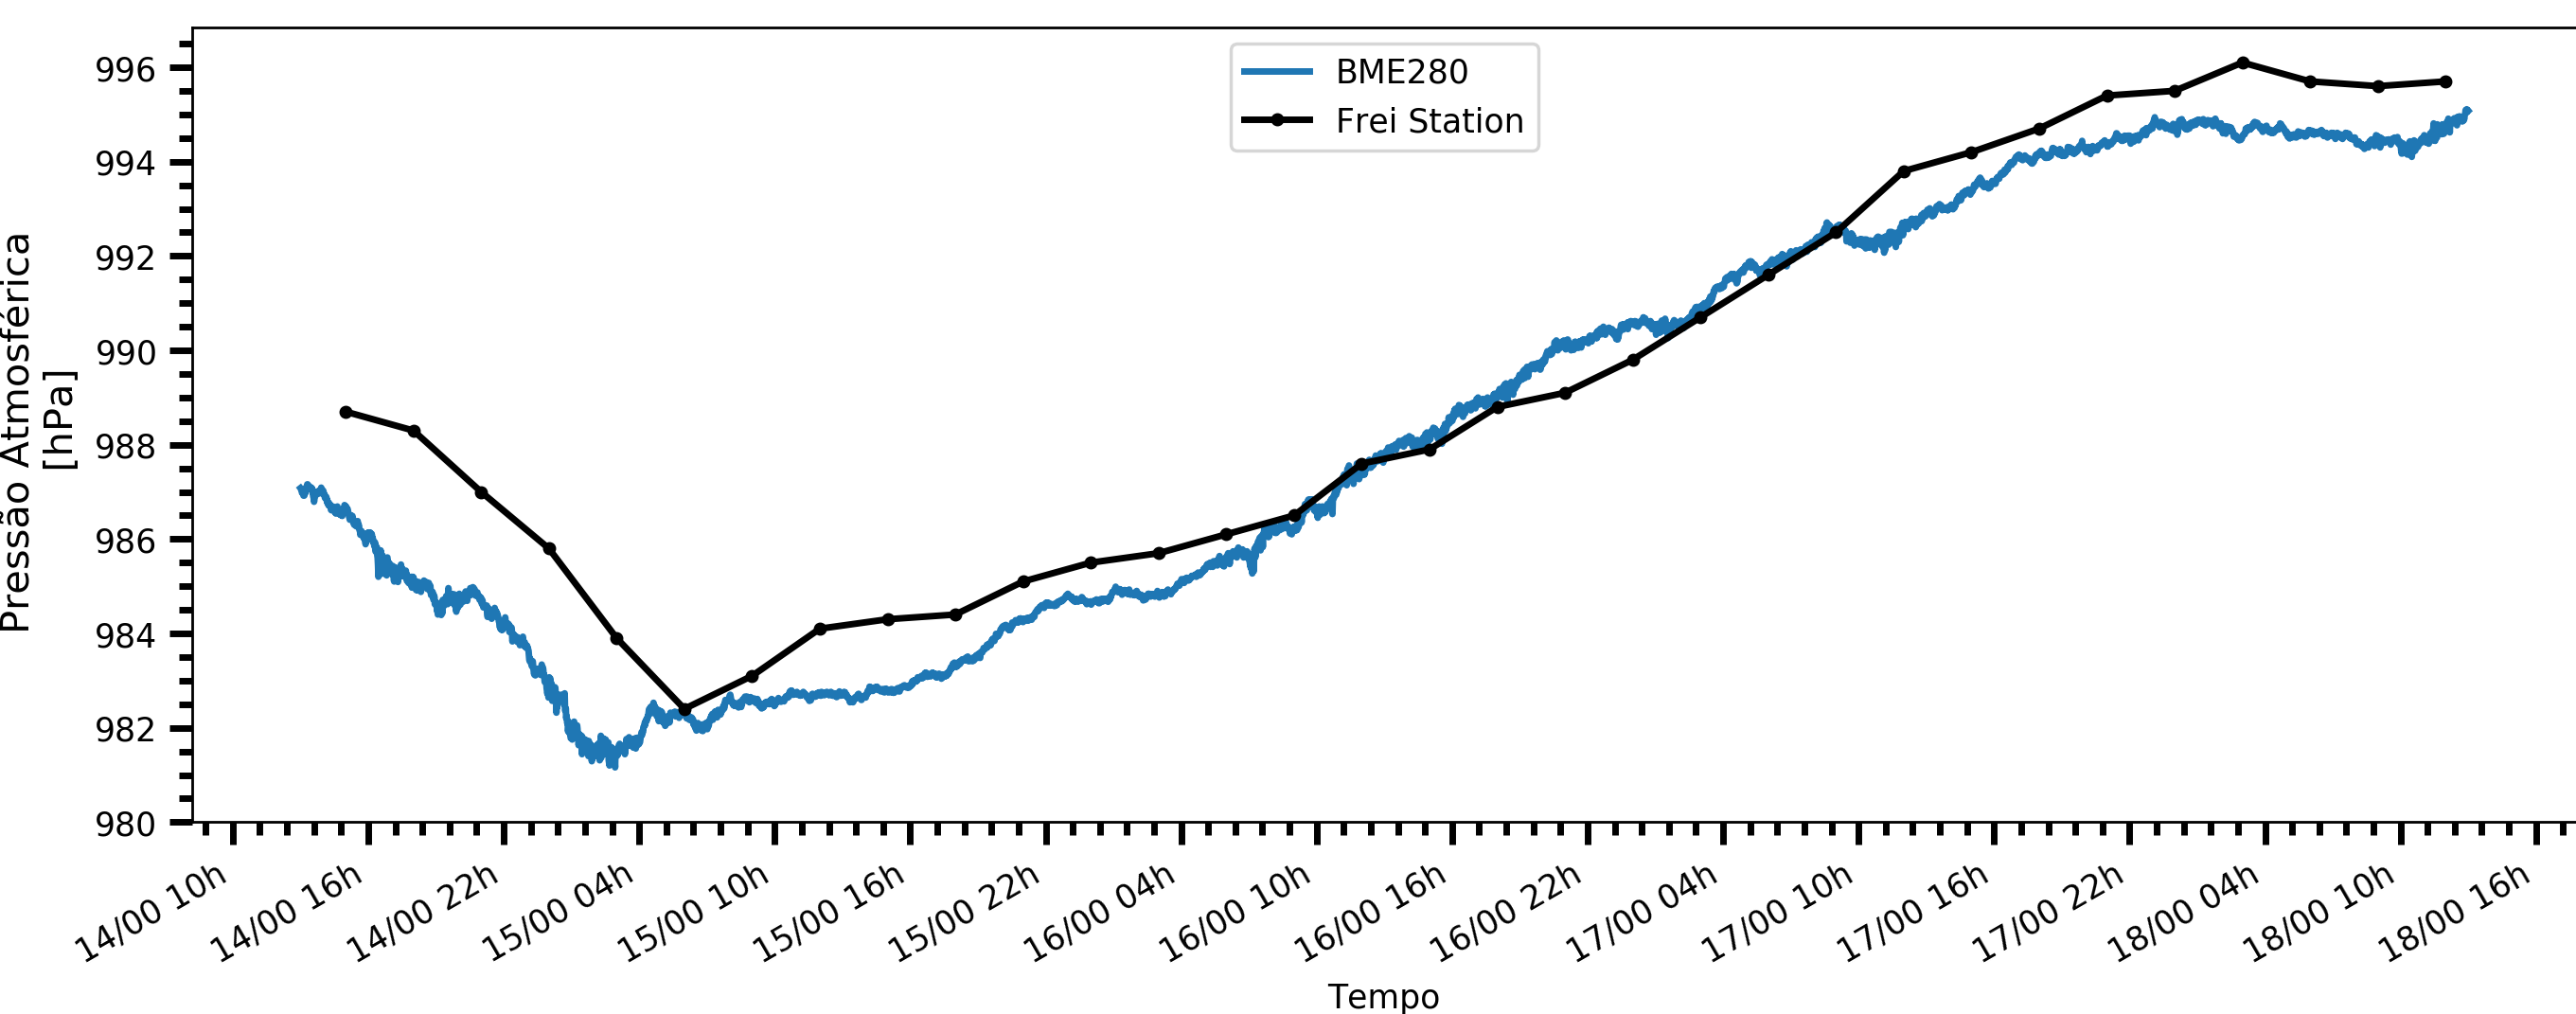
\includegraphics[width=0.70\textwidth]{img/dados.png}
	\caption{Pressão atmosférica na superfície coletada pelo DBCCDA (Azul) e pela Estação Chilena de Frei (Preto) entre os dias 14 e 18 de Fevereiro
	de 2020.}
	\label{dadosd}
\end{figure}
\bigskip

O segundo teste realizado, conforme a \textcolor{bleu_cite}{Figura \ref{dadosard2}}, comparou os dados de Temperatura do Ar (\textdegree{}C) e Pressão Atmosférica (hPa) do DBCCDA com os dados disponibilizados pelo
Instituto Nacional de Meteorologia (INMET) para a estação meteorológica A728, localizada entre -23.041668\textdegree{}S e -45.520841\textdegree{}O entre os 
dias 12 e 19 de Abril de 2020. É possível observar a destreza do DBCCDA em coletar dados similares aos coletados pela estação meteorológica. O RMSE calculado 
para a Temperatura do Ar entre os dois conjuntos de dados foi de 1.71 e com um p-valor menor que 0.001 e o r\textsuperscript{2} de 0.928. Os dados de Pressão Atmosférica (hPa)
também apresentaram uma grande simiridade entre os dois conjuntos, com um RMSE de 0.45, um p-valor menor que 0.001 e um r\textsuperscript{2} de 0.997.
\bigskip

\begin{figure}[H]
    \centering
    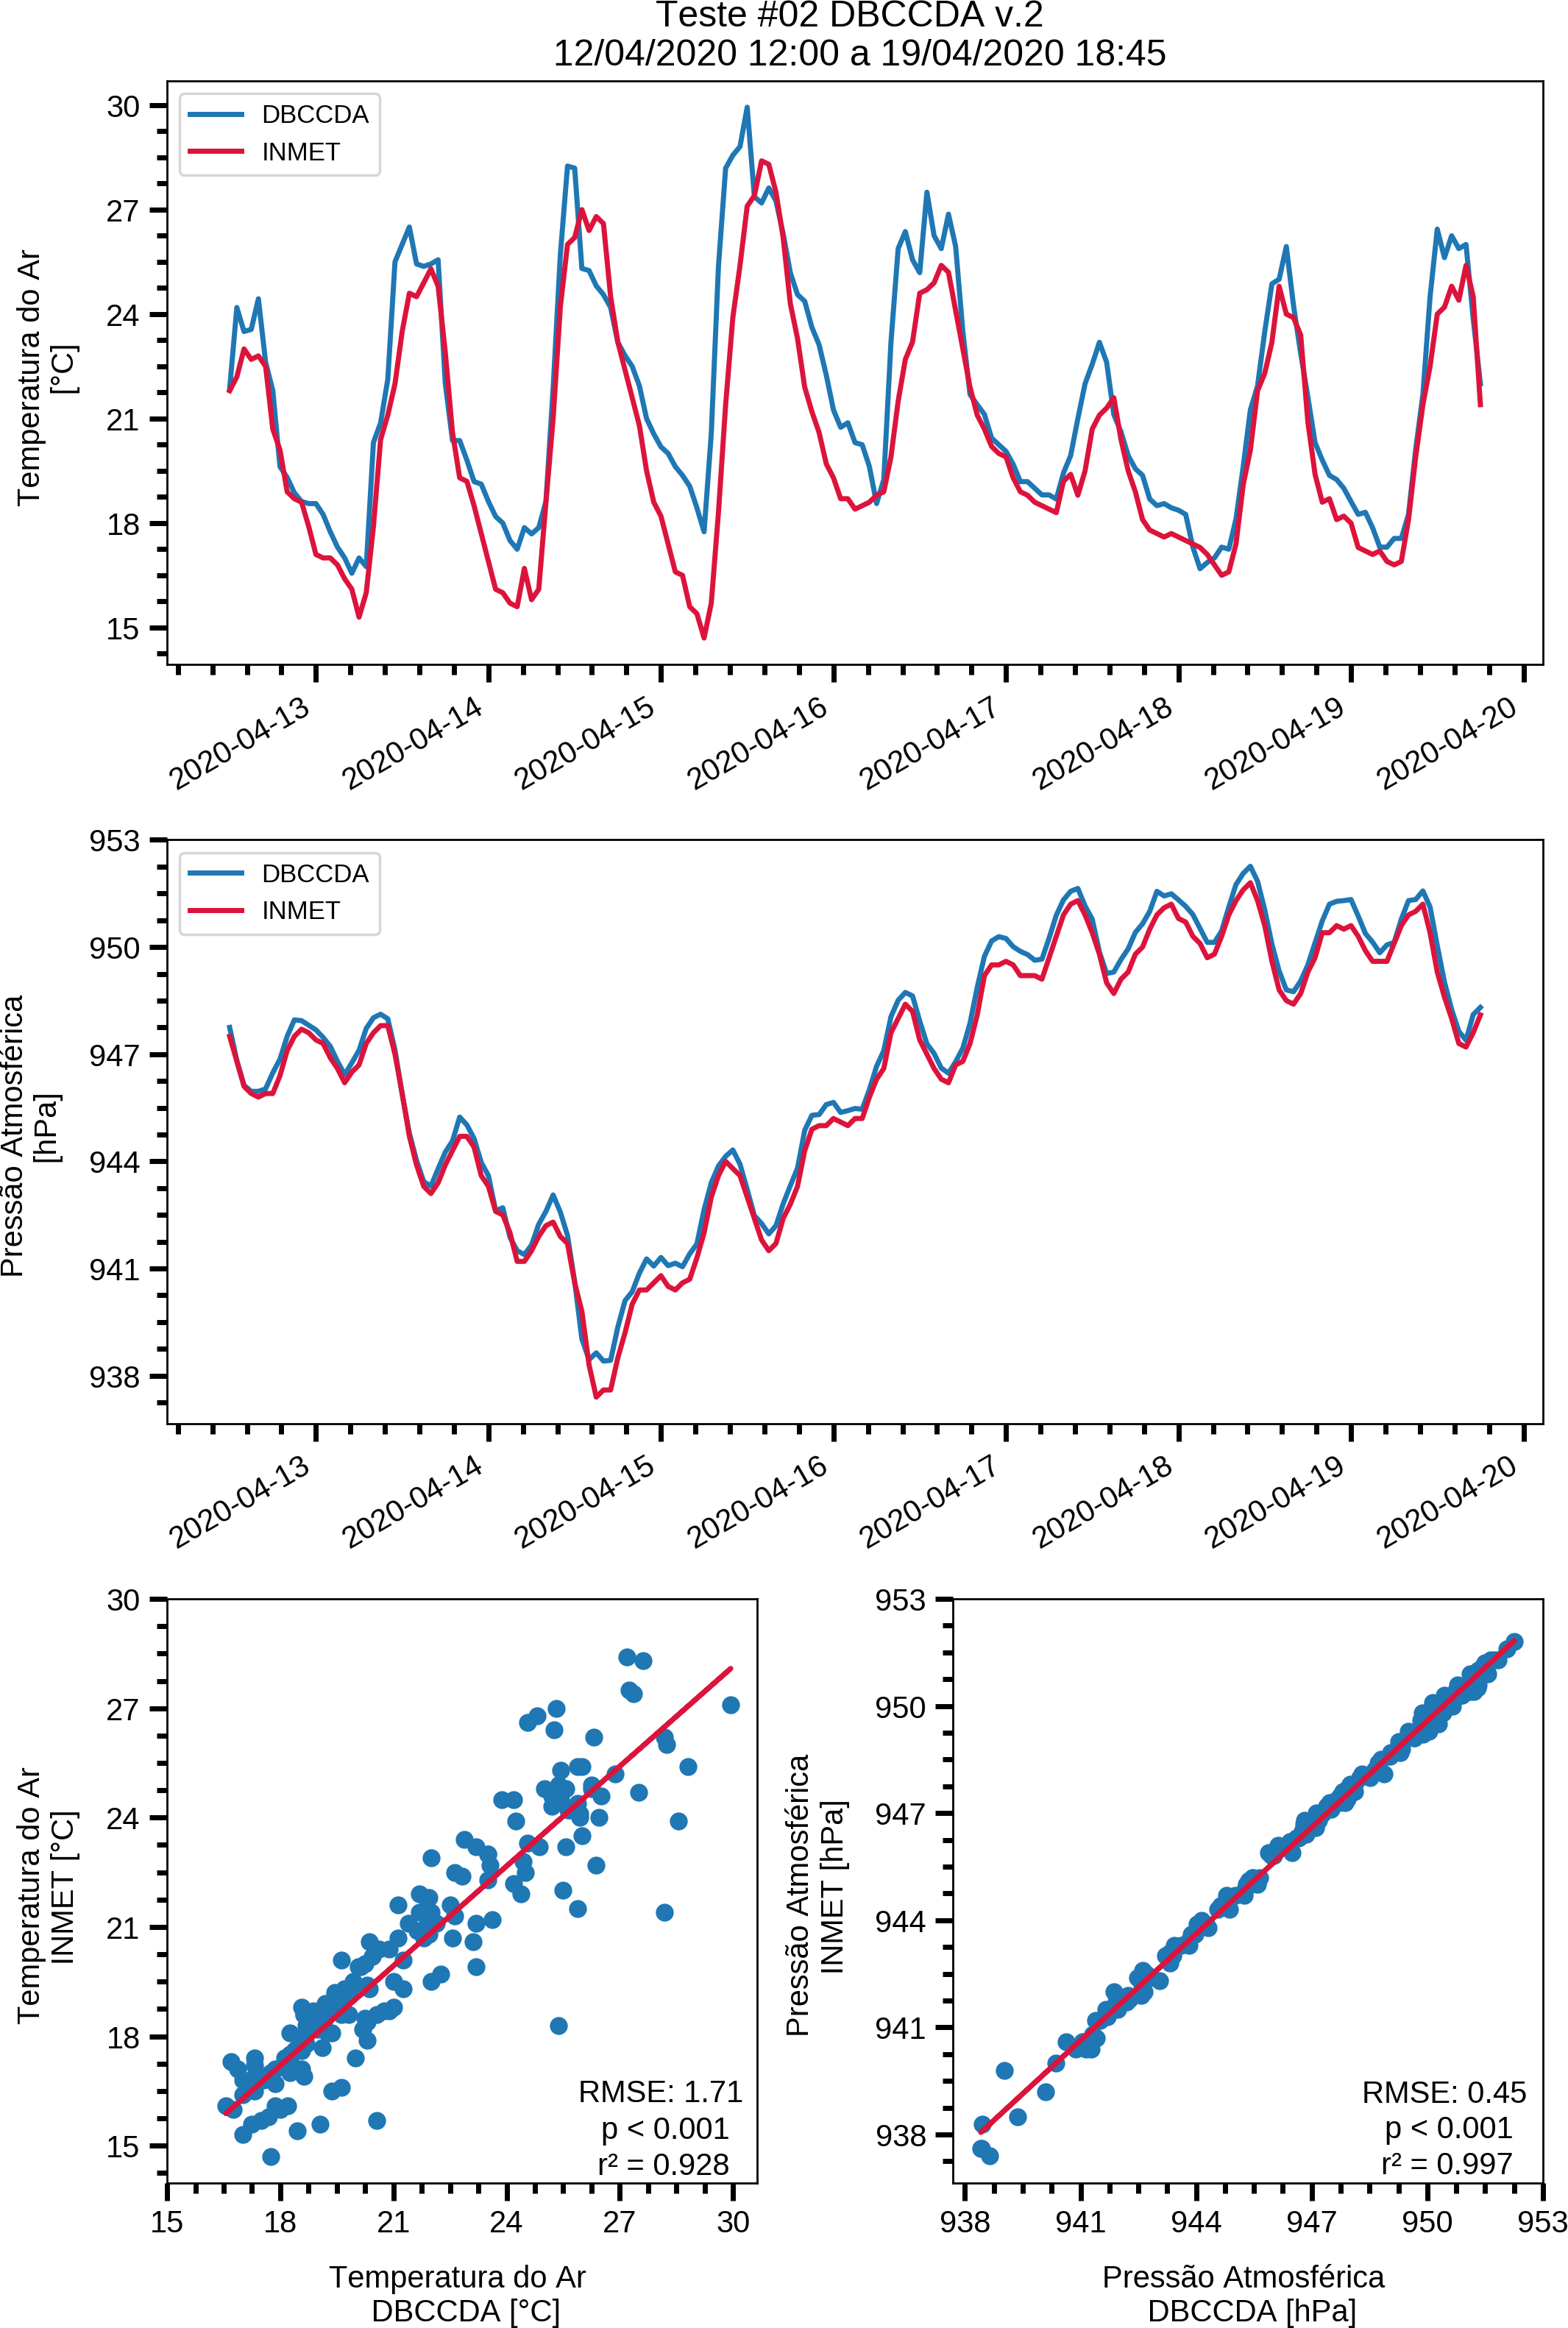
\includegraphics[width=0.60\textwidth]{img/xy_lcamd.png}
	\caption{Comparação dos dados de Pressão Atmosférica (hPa) e Temperatura do Ar (\textdegree{}C) coletados pelo DBCCDA (Azul) com os dados da estação meteorológica A728 do INMET (Vermelho)
	entre os dias 12 e 19 de Abril de 2020.}
	\label{dadosard2}
\end{figure}

\subsection{Resultados Esperados}
\bigskip

Espera-se ao longo da execução do projeto:

\begin{itemize}
	\item Ter um sistema de previsão do tempo e clima antártico operacional e confiável no INPE;
	\item Desenvolver um dispositivo de baixo custo que seja usado para coleta de dados atmosféricos na Antártica;
	\item Compreender melhor o comportamento da formação de massas de água no Mar de Weddell a partir da influência da existência ou não 
	do gelo marinho na superfície oceânica;
	\item Propor mecanismos físicos que expliquem o papel do oceano e da atmosfera na restauração do estado de equilíbrio do gelo marinho;
	\item Conhecer o impacto desempenhado pelo gelo marinho nos fluxos de calor, \textit{momentum} e massa na região do Mar de Weddell;
	\item Análise da persistência (dias ou meses) de uma condição de máxima concentração e espessura do gelo marinho antártico no Mar de Weddell; 
	\item Conhecer o impacto das correntes oceânicas no vento em superfície no Mar de Weddell a partir de simulações com e sem a presença de gelo marinho.
\end{itemize}

\section{PLANO DE TRABALHO E CRONOGRAMA DE EXECUÇÃO}
\bigskip

Propomos, a partir da \textcolor{bleu_cite}{Tabela \ref{cronos}}, os seguintes marcadores para o progresso do projeto de tese de doutorado:

\begin{enumerate}
	\item \label{a} Cumprimento das disciplinas do Doutorado;	
	\item \label{b} Cumprimento da Prova obrigatória de Línguas;
	\item \label{c} Preparação do projeto (Aquisição de dados \textit{in situ} do DBCCDA e compilação do modelo);
	\item \label{d} Primeiras simulações-teste do projeto e assimilação de dados do DBCCDA;
	\item \label{e} Execução das simulações numéricas utilizando o sistema acoplado COAWST;
	\item \label{f} Cumprimento do Exame de Qualificação;
	\item \label{g} Avaliação das simulações numéricas a partir de dados \textit{in situ} do DBCCDA e Sensoriamento Remoto;
	\item \label{h} Cumprimento do Exame de Proposta da Tese;
	\item \label{i} Análises das simulações - Cálculo dos Fluxos Turbulentos de Calor, massa e \textit{momentum};
	\item \label{j} Submissão de artigo para o Congresso do Scientific Committee on Antarctic Research (SCAR);
	\item \label{k} Submissão de artigo em revista Qualis-A;
	\item \label{l} Doutorado Sanduíche no exterior, com o Dr. John Warner da Woods Hole/USGS - EUA;
	\item \label{m} Submissão de artigo em revista Qualis-A internacional;
	\item \label{n} Defesa da tese de doutorado;
	\item \label{o} Embarque nas Operações Antártica para coletas de dados \textit{in situ};
	\item \label{p} Revisão bibliográfica da literatura.
\end{enumerate}

\begin{table}[H]
	\centering
	\begin{tabular}{|c|c|c|c|c|c|c|c|c|c|c|}
	\hline
	\multirow{2}{*}{\textbf{Atividades}} & \multicolumn{8}{c|}{\textbf{Cronograma de atividades: 2021-2024}}                                                                                                                                                                                                                                                                                                                                                                                                                                                                                                          \\ \cline{2-9} 
										 & \textbf{\begin{tabular}[c]{@{}c@{}}1º \\ sem. \\ 2021\end{tabular}} & \textbf{\begin{tabular}[c]{@{}c@{}}2º \\ sem. \\ 2021\end{tabular}} & \textbf{\begin{tabular}[c]{@{}c@{}}1º \\ sem.\\ 2022\end{tabular}} & \textbf{\begin{tabular}[c]{@{}c@{}}2º \\ sem.\\ 2022\end{tabular}} & \textbf{\begin{tabular}[c]{@{}c@{}}1º \\ sem. \\ 2023\end{tabular}} & \textbf{\begin{tabular}[c]{@{}c@{}}2º \\ sem.\\ 2023\end{tabular}} & \textbf{\begin{tabular}[c]{@{}c@{}}1º \\ sem. \\ 2024\end{tabular}} & \textbf{\begin{tabular}[c]{@{}c@{}}2º \\ sem. \\ 2024\end{tabular}} \\ \hline
    \textbf{\ref{a}}                     & \cellcolor{bleu_cite}                                               & \cellcolor{bleu_cite}                                               &                                                                    &                                                                    &                                                                     &                                                                    &                                                                    &                                                                      \\ \hline
    \textbf{\ref{b}}                     & \cellcolor{bleu_cite}                                               &                                                                     &                                                                    &                                                                    &                                                                     &                                                                    &                                                                    &                                                                      \\ \hline
	\textbf{\ref{c}}                     & \cellcolor{bleu_cite}                                               &                                                                     &                                                                    &                                                                    &                                                                     &                                                                    &                                                                    &                                                                      \\ \hline
	\textbf{\ref{d}}                     & \cellcolor{bleu_cite}                                               & \cellcolor{bleu_cite}                                               &                                                                    &                                                                    &                                                                     &                                                                    &                                                                    &                                                                      \\ \hline
	\textbf{\ref{e}}                     &                                                                     & \cellcolor{bleu_cite}                                               &                                                                    &                                                                    &                                                                     &                                                                    &                                                                    &                                                                      \\ \hline
	\textbf{\ref{f}}                     &                                                                     &                                                                     & \cellcolor{bleu_cite}                                              &                                                                    &                                                                     &                                                                    &                                                                    &                                                                      \\ \hline	
	\textbf{\ref{g}}                     &                                                                     &                                                                     & \cellcolor{bleu_cite}                                              &                                                                    &                                                                     &                                                                    &                                                                    &                                                                      \\ \hline
	\textbf{\ref{h}}                     &                                                                     &                                                                     &                                                                    & \cellcolor{bleu_cite}                                              &                                                                     &                                                                    &                                                                    &                                                                      \\ \hline	
	\textbf{\ref{i}}                     &                                                                     &                                                                     &                                                                    & \cellcolor{bleu_cite}                                              & \cellcolor{bleu_cite}                                               &                                                                    &                                                                    &                                                                      \\ \hline
	\textbf{\ref{j}}                     &                                                                     &                                                                     &                                                                    &                                                                    &                                                                     & \cellcolor{bleu_cite}                                              &                                                                    &                                                                      \\ \hline
	\textbf{\ref{k}}                     &                                                                     &                                                                     &                                                                    &                                                                    &                                                                     & \cellcolor{bleu_cite}                                              &                                                                    &                                                                      \\ \hline
	\textbf{\ref{l}}                     &                                                                     &                                                                     &                                                                    &                                                                    &                                                                     & \cellcolor{bleu_cite}                                              & \cellcolor{bleu_cite}                                              &                                                                      \\ \hline
	\textbf{\ref{m}}                     &                                                                     &                                                                     &                                                                    &                                                                    &                                                                     &                                                                    & \cellcolor{bleu_cite}                                              &                                                                      \\ \hline
	\textbf{\ref{n}}                     &                                                                     &                                                                     &                                                                    &                                                                    &                                                                     &                                                                    &                                                                    & \cellcolor{bleu_cite}                                                \\ \hline
	\textbf{\ref{o}}                     &                                                                     & \cellcolor{bleu_cite}                                               &                                                                    & \cellcolor{bleu_cite}                                              &                                                                     &                                                                    &                                                                    & \cellcolor{bleu_cite}                                                \\ \hline
	\textbf{\ref{p}}                     & \cellcolor{bleu_cite}                                               & \cellcolor{bleu_cite}                                               &  \cellcolor{bleu_cite}                                             & \cellcolor{bleu_cite}                                              & \cellcolor{bleu_cite}                                               & \multicolumn{1}{l|}{\cellcolor{bleu_cite} }                        & \multicolumn{1}{l|}{\cellcolor{bleu_cite}}                        & \multicolumn{1}{l|}{\cellcolor{bleu_cite}}                           \\ \hline
	
\end{tabular}
\caption{Cronograma de atividades desenvolvida para o projeto de tese de doutorado.}
\label{cronos}
	\end{table}

%%% Considerações finais
\section{CONSIDERAÇÕES FINAIS}
\bigskip

Este projeto de doutorado faz parte de uma iniciativa inovadora e promissora que visa contribuir para um  
melhor entendimento dos processos dinâmicos e termodinâmicos de interação do gelo marinho-oceano-atmosfera  
no setor Atlântico do Oceano Austral. Espera-se aprofundar o conhecimento sobre o impacto do gelo marinho na atmosfera
e no oceano.

Através da análise dos resultados, espera-se avançar no entendimento dos modos de variabilidade oceânica e 
atmosférica dos fluxos de calor e \textit{momentum} e seus processos associados, assim como os impactos eventuais desses processos 
na região de estudo. Nessa proposta, uma forte ênfase foi dada ao desenvolvimento de um modelo regional acoplado, 
que considere as componentes de gelo marinho, oceano, ondas e atmosfera e que já é dominada pelos proponentes do projeto.
Esta ferramenta será empregada no estudo dos processo dinâmicos e termodinâmicos que ocorrem nestas interfaces. Os dados 
observacionais \textit{in  situ}, coletados anualmente nas Operações Antárticas do Projeto ATMOS, também serão de extrema  
valia para a utilização em conjunto com o sistema de modelagem, pois permitirá fazer ajustes e verificações da destreza dos
modelos e auxiliarão no ajuste fino das parametrizações físicas. Espera-se ao fim do projeto poder contar com um sistema 
regional acoplado de modelagem numérica, que disponha de altíssima resolução para auxiliar em outras atividades de pesquisa 
ou até mesmo rotinas operacionais de previsão tempo e clima no Instituto Nacional de Pesquisas Espaciais. 

Espera-se que a análise integrada dos fenômenos regionais estudados com o auxílio de ferramentas de modelagem  
numérica e com dados \textit{in situ} possa garantir, no futuro, um melhor entendimento dos processos físicos que ocorrem na  
região de estudo. A expectativa é que eventualmente este conhecimento possa ajudar na melhora dos esquemas  de  
simulação e previsão do tempo e clima para a região desse estudo. Unindo-se a dados e resultados de outros projetos
em andamento, os gerados por essa proposta contribuirão para que o entendimento de fenômenos com origem em altas 
latitudes que serão revertidos numa melhor compreensão dos fenômenos oceânicos e atmosféricos de maior escala.

%%% Bibliografia
\linespread{1}
\printbibliography[ heading=bibintoc, title={REFERÊNCIAS BIBLIOGRÁFICAS}]

\end{document}